%% ----------------------------------------------------------------
%% Currentwork.tex
%% ---------------------------------------------------------------- 
\chapter{Energy Storage and Harvester Sizing for Deploying Intermittently-Powered IoT Devices} \label{Chapter:Work1}

\setlength{\headheight}{26pt}

\section{Motivations}

\textbf{Sizing concerns for energy storage.} In order to minimise device dimensions, published works in intermittent computing typically only adopt a minimum amount of energy storage, which is just enough for decoupling or ensuring computing correctness. Unfortunately, given power production is less than power consumption, a storage-less system has to frequently wake up, execute shortly, and halt, consuming much energy in managing system states. Provisioning more energy storage prolongs such operating cycles, and hence, reduces the overheads of saving and restoring state. However, increasing storage also comes with prices. Oversized capacitors typically manifest high leakage compared to low-power devices, draining usable energy. Therefore, storage-less intermittent computing systems suffer from frequent state managing operations, while oversized storage introduce high leakage. Either case reduces the energy spent in effective execution, affecting application performance. 

\textbf{Sizing concerns for energy harvester.} 
The size of energy harvester is determined at design time and has a positive relation with the power production. How to determine the energy harvester size largely depends on the priority of design requirements. There are typically two design requirements: minimum average performance and maximum device dimensions. If minimum average performance should be met, the smallest harvester size that just satisfies this performance should be chosen in order to minimise dimensions. If maximum device dimensions should be met, the largest harvester size under this limit should be chosen in order to maximise performance. If both requirements can be met at the same time, which means there is a range of available harvester sizes, a balance between these two requirement should be considered. 

Equilibrium exists between performance and dimensions in energy storage and harvester sizing for intermittently-powered devices. To solve this sizing problem, we provide a sizing method that evaluates the relationship among the average performance, the storage capacity, the harvester dimensions. This sizing method takes energy condition data and generates a performance distribution by conversion functions from energy conditions to estimated performance. We demonstrate this sizing method in an intermittent computing device model powered by photovoltaic (PV) cells under outdoor deployment. In this example, we further analyse the sizing effects on system behaviours, with results showing that properly sizing energy storage leads to a performance increase by 5.7-22.2\% in a suggested range of energy harvester sizes under real-world deployment.



\section{Sizing Method for Energy Storage and Energy Harvester}

The goal of our sizing method is to generate the application performance given different energy storage capacities and energy harvester sizes, with a reference of actual dimensions. The result is then used to determine how to deploy energy storage and harvester with respect to specific design requirements for different application scenarios. This sizing method considers two aspects: estimating performance distribution and balancing device dimensions. 

\subsection{Estimating Performance Distribution}

In IoT deployment, performance is represented as the speed of application completion (denoted as $S_{app}$), e.g. the number of application iterations per second. The performance distribution under real-world deployment indicates how much time the device operates in each performance level and is helpful for judging whether the device meets performance requirements after deployment (the measurement for this depends on specific design considerations, which can be average performance or the performance at a certain percentile). 

To estimate the performance distribution after device deployment, our sizing method requires three inputs:  

\begin{itemize}
    \item $T_{ratio} = f(E_{source})$: The time length ratios of each energy source condition (intensity) $E_{source}$. 
    \item $P_{harvest} = f(E_{source})$: The conversion function from energy conditions to harvested power $P_{harvest}$. 
    \item $S_{app} = f(P_{harvest})$: The conversion function from harvested power to application performance $S_{app}$. 
\end{itemize}

As shown in Figure \ref{Figure:here}, $T_{ratio}= f(E_{source})$ is converted by $P_{harvest} = f(E_{source})$ into a harvested power distribution $T_{ratio} = f(P_{harvest})$. The $P_{harvest}$ distribution is then converted by $S_{app} = f(P_{harvest})$ into a performance distribution $T_{ratio} = f(S_{app})$ as a result. 

\begin{figure}[H]
    \centering
    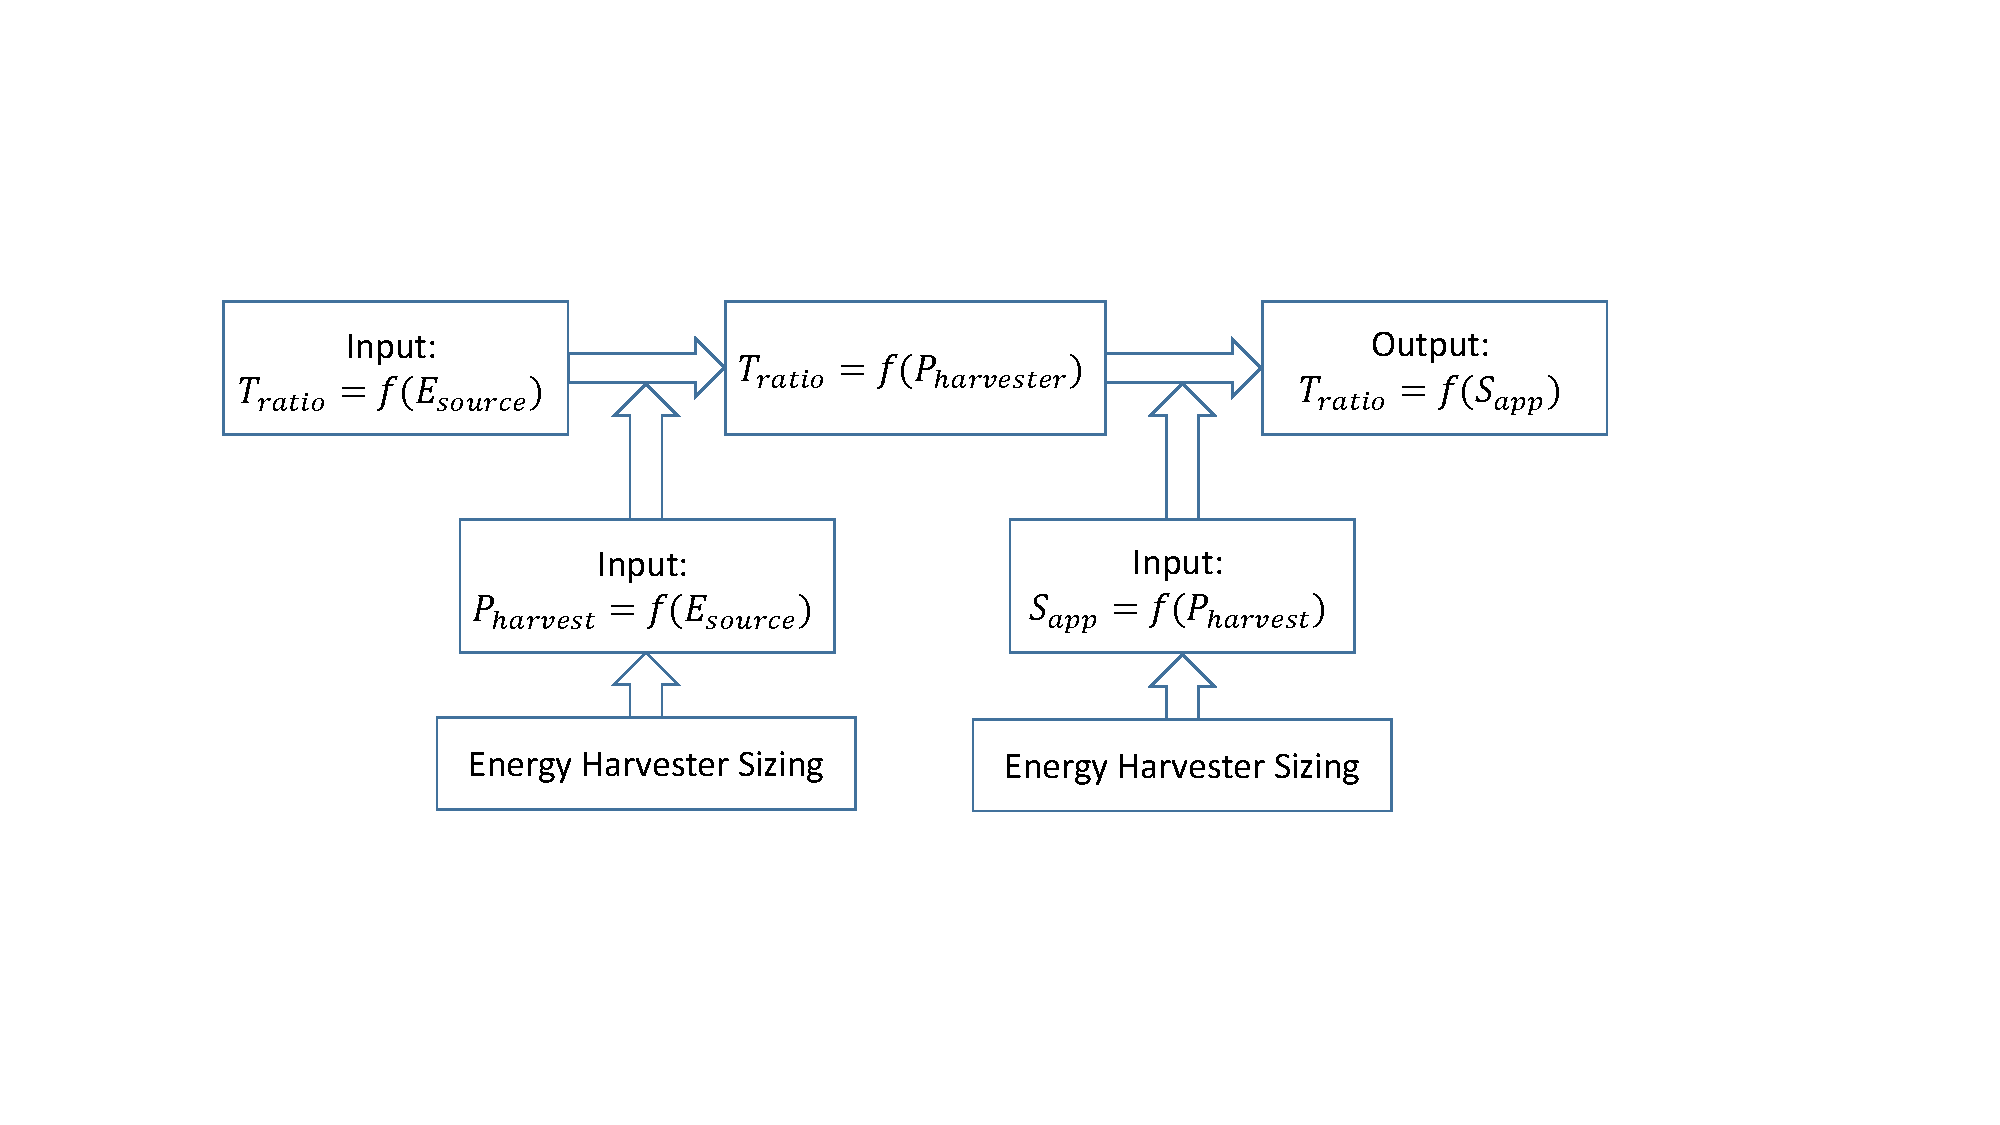
\includegraphics[width=13cm]{figure/work1/sizingmethod}
    \caption{Principles of the proposed sizing method.}
    \label{Figure:here}
\end{figure}

$T_{ratio} = f(E_{source})$ provides the predicted distribution of energy source conditions after deployment. In our implementation of solar energy harvesting devices, we use empirical annual solar irradiance data at the deployed location under an assumption that the solar irradiance at one location is similar each year. Alternative energy source prediction methods for this input can be also used. $P_{harvest} = f(E_{source})$ transduces the energy source to power supply. This can be obtained by modelling or measuring the output characteristics of the target energy harvester given a range of energy conditions. Sizing energy harvester has an effect on this energy transduction, because a larger harvester typically leads to more harvested power and vice versa. $S_{app} = f(P_{harvest})$ provides the relationship between the power supply and the delivered performance in intermittent computing devices. Sizing energy storage has an effect on this relationship. This is illustrated in Section \ref{Section:4.2} with formulations considering the fundamental behaviours of intermittent computing devices. 

\subsection{Balancing Device Dimensions}

In IoT deployment, the dimensions of devices become a concerned factor in size-constrained application scenarios, such as such as implantable sensors \cite{5627952}, healthcare \cite{6579688}, building automation \cite{6064380}. For energy storage and energy harvester sizing, the dimensional scale should be also considered. 
% wearables, smart cities, and healthcare

For energy storage, we find that properly sizing storage capacity in intermittent computing improves application performance given the same harvested power. This optimal storage may have a larger capacity than the minimum one (which is just enough for decoupling or ensuring computing correctness). However, dimensions also typically increase with storage capacity. Designers can choose a storage capacity that maximises performance while still meets their dimensional requirements. Our example in Section \ref{Section:4} shows that this optimal capacity does not significantly affect dimensions.
% This capacity-dimension relationship of energy storage is typically non-linear. 

For energy harvester, scaling dimensions typically increases or decreases harvested power linearly. Given the same ambient energy intensity, the power production of energy harvester is related to how large the part that interacts with the energy source is. For example, in light energy harvestering, the generated power is linear to the area of PV cells. However, although the size of energy harvester linearly contributes to the harvested power, the harvested power does not linearly lead to performance changes in energy harvesting devices under real-world deployment. A device has its maximum power consumption, above which the excessive harvested power cannot be consumed on effective execution. Also, under real-world deployment, the energy source intensity may spread over a wide spectrum over time, with some "high-energy" periods that provide enough power for devices to operate continuously. For such high-energy periods, increasing the harvester size does not provide execution speedup. 

% transition needed here. explain how to determine energy harvester size, with respect to the other two "easy" goals.

To evaluate an efficient energy harvester size, we introduce \textit{performance per space} (P/S ratio) as a measurement to indicate how effectively the harvester dimensions contribute to application performance. A high P/S ratio indicates the allocated harvester size is effectively transduced into application performance. Designers can choose a harvester within a nearly maximum range according to their requirements for performance or dimensions. Harvester sizes outside this "nearly maximum" range can be still chosen if needed.



\section{Modelling Intermittent Computing Systems}

\subsection{Model Overview}

We build a time-traversing model to explore the power and performance behaviours of intermittent computing systems and demonstrate our sizing method.

The framework of our model is shown in Figure \ref{Figure:framework}. With the focus on the sizing effect of energy harvester and energy storage, this model has mainly four components: \textit{Energy Source}, \textit{Energy Harvester}, \textit{Energy Storage}, and \textit{Load}. \textit{Energy Source} inputs a trace of time-varying energy source intensity. The other three, i.e. \textit{Energy Harvester}, \textit{Energy Storage}, and \textit{Load}, constitute an energy harvesting sensor system. A typical load of energy harvesting sensing devices consists of a microcontroller unit (MCU) and peripherals (e.g. sensors and a radio).

\begin{figure}[H]
    \centering
    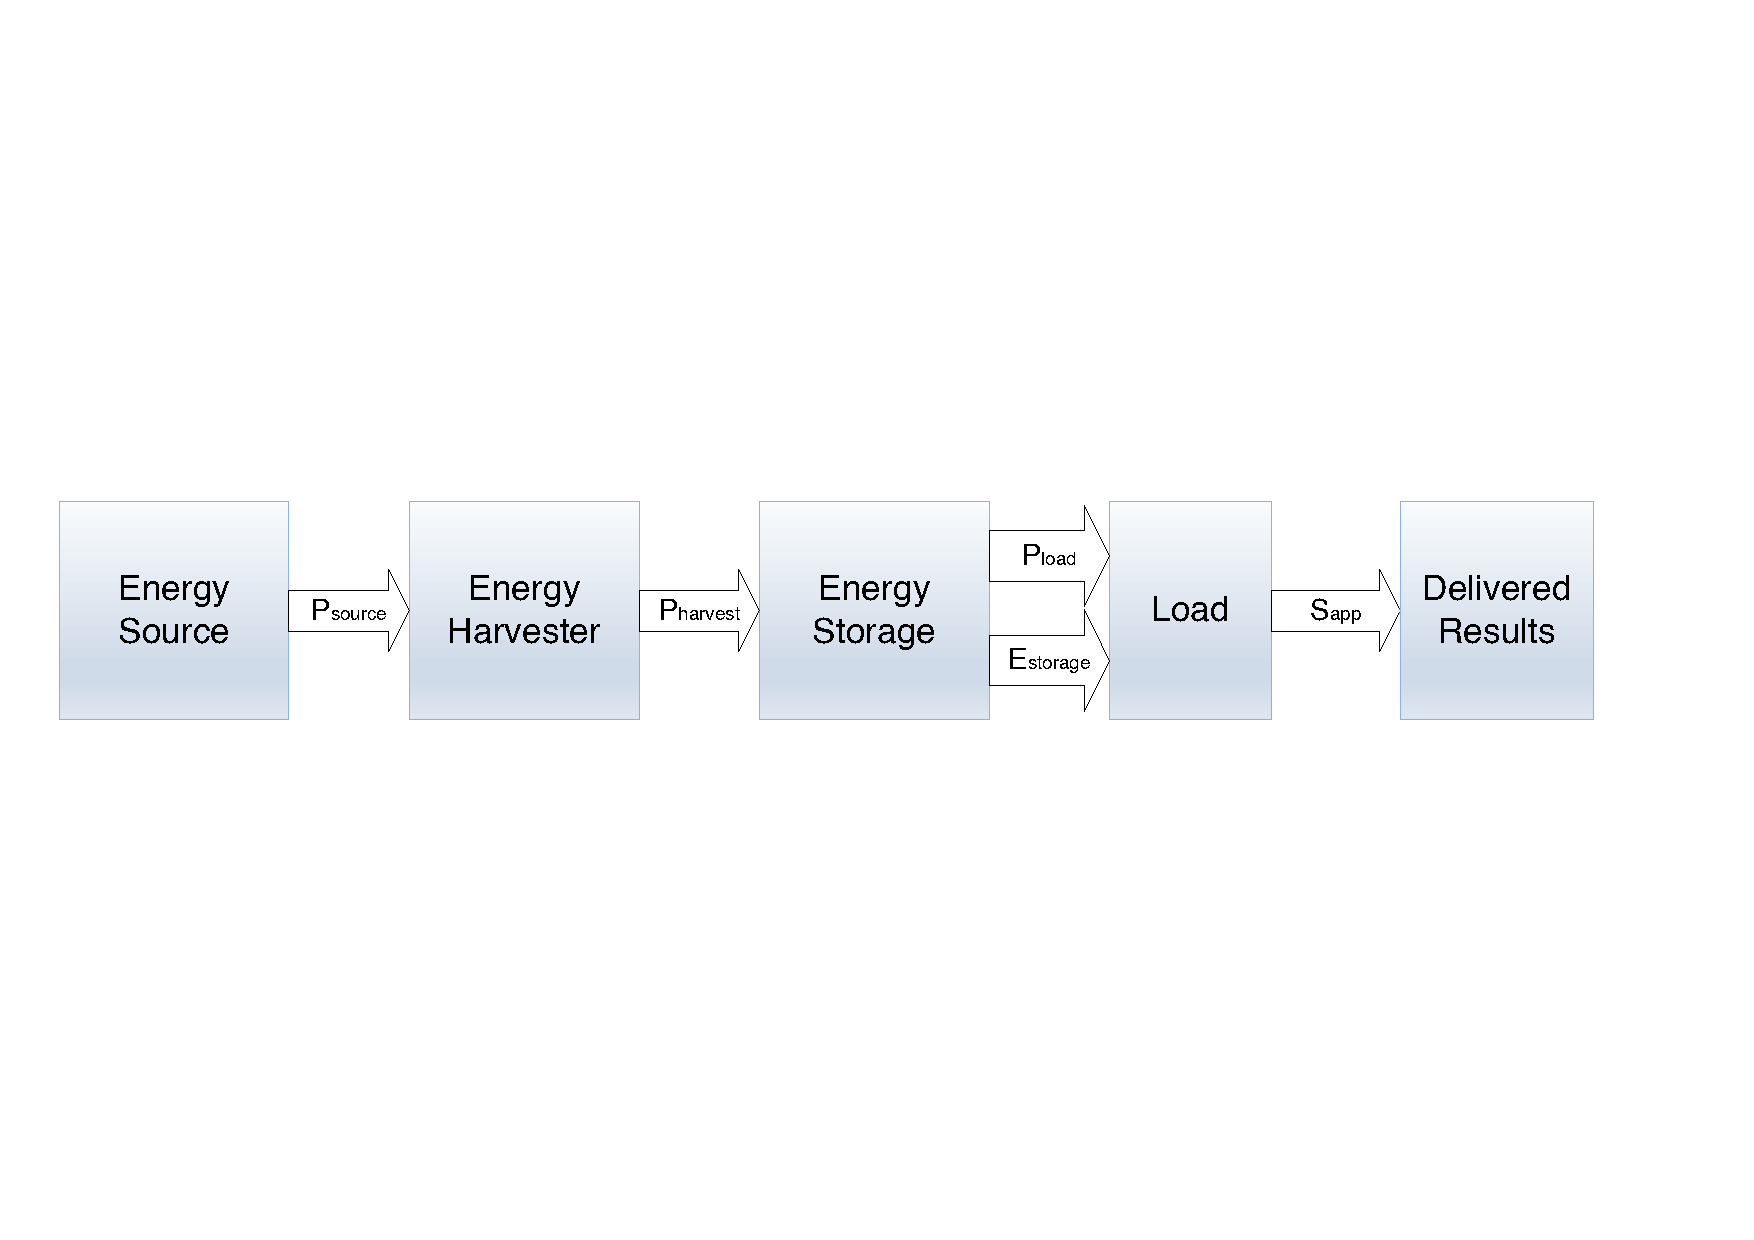
\includegraphics[width=15cm]{figure/work1/model}
    \caption{Model framework.}
    \label{Figure:model}
\end{figure}

We apply this model framework to an outdoor solar energy harvesting device. As shown in Figure \ref{Figure:framework}, the four modules are implemented by solar irradiance, a PV module, a capacitor, and an MCU. The latter three forms the device, and are mutually linked by current flows $I_{harvest}$ and $I_{load}$ and operating voltage $V_{cc}$. The major parameters (outputs of modules) are listed in Table \ref{Table:parameter}. We omit thermal effects in this model and assume that the system working temperature is 25 $^{\circ}$C.
% \dots explain more about how each module link together, and a high-level framework
% \dots talk about our own example. why couple Vcc to harvester and load

\begin{figure}[H]
    \centering
    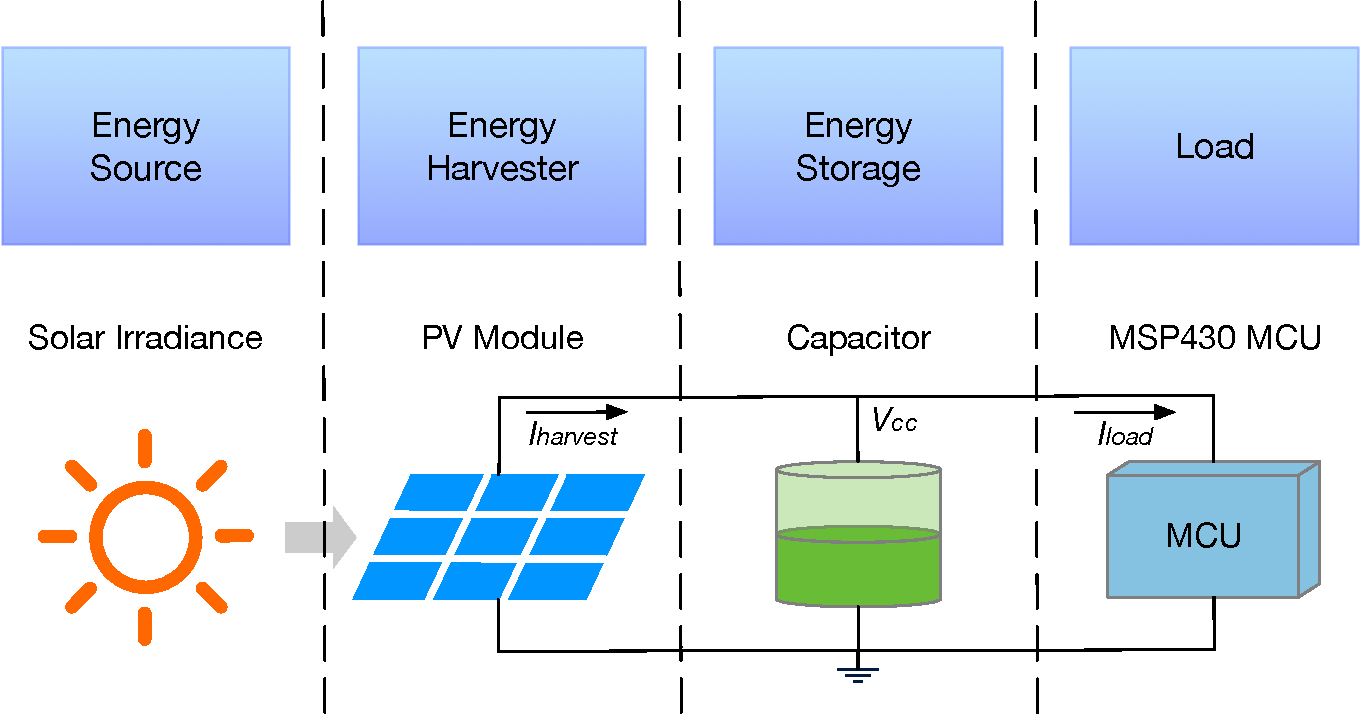
\includegraphics[width=15cm]{figure/work1/framework}
    \caption{An outdoor solar energy harvesting device model, with high-level modules (upper) and the example components selected for each module (lower).}
    \label{Figure:framework}
\end{figure}

\begin{table}[H]
\caption{Major input and output parameters of modules.}
\label{Table:parameter}
\centering
%% \tablesize{} %% You can specify the fontsize here, e.g., \tablesize{\footnotesize}. If commented out \small will be used.
\begin{tabular}{ccc}
\toprule
\textbf{Module}	& \textbf{Parameter} & \textbf{Description} \\
\midrule
Energy Source & $G$ & Solar irradiance \\
\midrule
% \multirow{2}{*}{Energy Harvester} & $I_{harvest}$ & Harvested current\\
% & data & data\\
\multirow{2}{*}{Energy Harvester} & $I_{harvest}$ & Harvested current \\
& $A_{cell}$ & PV cell area \\
\midrule
\multirow{2}{*}{Energy Storage} & $V_{cc}$ & System operating voltage \\
& $C$ & Capacitance \\
\midrule
\multirow{2}{*}{Load} & $I_{load}$ & Load current consumption \\
& $S_{app}$ & Application performance \\
\bottomrule
\end{tabular}
\end{table}

\subsection{Energy Source and Harvester} \label{Section:3.2}

The energy harvester explored in this work is a PV panel, with outdoor solar energy as the energy source. 

The energy source intensity is represented as a time-varying irradiance trace. This trace is defined by irradiance as a function of time. The real-world solar irradiance dataset we used in this work is taken from NREL Solar Radiation Research Laboratory \cite{stoffel1981nrel}, which records outdoor solar irradiance traces of several years at multiple locations. We choose the global horizontal irradiance data as the energy source input.

In terms of the energy harvester, we picked a recently developed model of PV cells proposed by Vergura S. \cite{en9050326}. This model takes the parameters available in the datasheets of common PV cells, so it is convenient to reconfigure and suit different types of PV cells. In this PV cell model, the output current of PV cells is expressed as: 

\begin{equation} \label{Equation:pvcell}
    I_{harvest} = \frac{G}{G_{ref}} I_{sc} (1 - (1 - \frac{I_{mpp}}{I_{sc}}) ^ {\frac{V_{cc}-V_{oc}}{V_{mpp} - V_{oc}}})
\end{equation}

where $V_{cc}$ is the operating voltage of the PV cell, $G$ is the input irradiance, $G_{ref}$ is the reference irradiance which is normally 1000$W/m^2$, and $I_{sc}$, $V_{oc}$, $I_{mpp}$, $V_{mpp}$ are short-circuit current, open-circuit voltage, current and voltage at maximum power point (MPP) respectively given the reference irradiance. $V_{cc}$ and $G$ are dynamic conditions at run time, while other parameters are fixed at design time and set according to datasheets. 

The short-circuit current $I_{sc}$ of a PV panel is proportional to the area of each cell, and the open-circuit voltage $V_{oc}$ of a PV panel is proportional to the number of cells in series. We refer to Panasonic "Amorton" amorphous silicon solar cells \cite{solarcell} for PV cell settings, as shown in Table \ref{Table:pvcell}. To match the maximum operating voltage 3.6V of our load (Section \ref{load}), the number of cells in series is set to four (with $V_{oc}$ = 3.56V) for the following tests. When the area of cells changes, $I_{sc}$ and $I_{mpp}$ change linearly. According to Equation \ref{Equation:pvcell}, sizing the PV cells scales the harvested current $I_{harvest}$ linearly as $I_{mpp} / I_{sc}$ maintains constant and $I_{sc}$ is linearly to the cell area. 

\begin{table}[H]
    \caption{PV Cell Properties under AM1.5 1000W/m$^2$ Light Conditions.}
    \label{Table:pvcell}
    \centering
    \begin{tabular}{ccc}
    \toprule
    \textbf{Property} & \textbf{Value} \\
    \midrule
    Open-Circuit Voltage & 0.89 V/cell \\
    Short-Circuit Current & 14.8 mA/cm$^2$ \\
    MPP Voltage & 0.65 V/cell \\ 
    MPP Current & 12.1 mA/cm$^2$ \\
    \bottomrule
    \end{tabular}
\end{table}

\subsection{Energy Storage}

The energy storage is modelled as an electrolytic capacitor with capacitance-related leakage. The terminal voltage of this capacitor is also the operating voltage for the PV panel and the load, this voltage can be expressed as

\begin{equation}
    dV_{cc} = \frac{I_{harvest} - I_{load} - I_{leak}}{C} dt
\end{equation}

where $I_{load}$ is the current consumption of the load, and $I_{leak}$ is the current leakage of the capacitor itself, $C$ is the capacitance. To model this leakage, we refer to the datasheet of an aluminum capacitor \cite{alcapacitor}, in which the current leakage of this capacitor is given as:

\begin{equation}
    I_{leak} = max\{0.03 C V_{rated}, \quad 4 \times 10^{-6}\} \quad (A)
\end{equation}

where $V_{rated}$ is the rated voltage of the capacitor, which is 10 V in our model. 

Here, $V_{cc}$ affects both the energy harvester and the load. On the harvester side, $V_{cc}$ is the operating voltage of PV cells, which has an effect on the harvested current $I_{harvest}$. On the load side, $V_{cc}$ is the supply voltage, which determines when the load wakes up or powers off (affecting $I_{load}$). Hence, the energy storage, the energy harvester, and the load impact on each other through $V_{cc}$, $I_{harvest}$, and $I_{load}$. 

\subsection{Load} \label{load}

This part aims to model power consumption and application performance of intermittent computing loads. Intermittent computing is achieved by maintaining system computing states consistent over power failures. A computing state includes program counter, processor registers, cache, and RAM data, etc. Intermittent computing devices save and restore computing states either at pre-installed points (known as proactive approaches) or when a power failure is imminent (known as reactive approaches). As the behaviours of proactive systems depends largely on how to insert state-saving points in the program, we use reactive systems as the load model in our exploration. 

% Execution routine. 
The flowchart in Figure \ref{Figure:routine} explains the system control routine of a reactive intermittent computing system \cite{6960060}. There are three typical voltage thresholds in such systems, $V_{off}$, $V_{save}$, and $V_{restore}$ ($V_{off} < V_{save} < V_{restore}$). When the supply voltage is available ($V_{cc} > V_{off}$), the system first stays in sleep mode until $V_{cc} > V_{restore}$. After that, the system checks if there is a saved state. If there is, the state is restored from NVM and the program continues from the last interrupted point; otherwise, the program starts from the beginning of application. The execution continues until $V_{cc} < V_{save}$, which indicates an imminent power failure and triggers a state-saving operation. During the saving operation, the current state is saved into NVM and then the system sleeps. If $V_{cc}$ recovers to $V_{restore}$ again, the system exits sleep mode and resumes execution without the need for restoring; otherwise, if $V_{cc}$ keeps dropping to $V_{off}$, the system powers off and the volatile state is lost.

\begin{figure}[H]
    \centering
    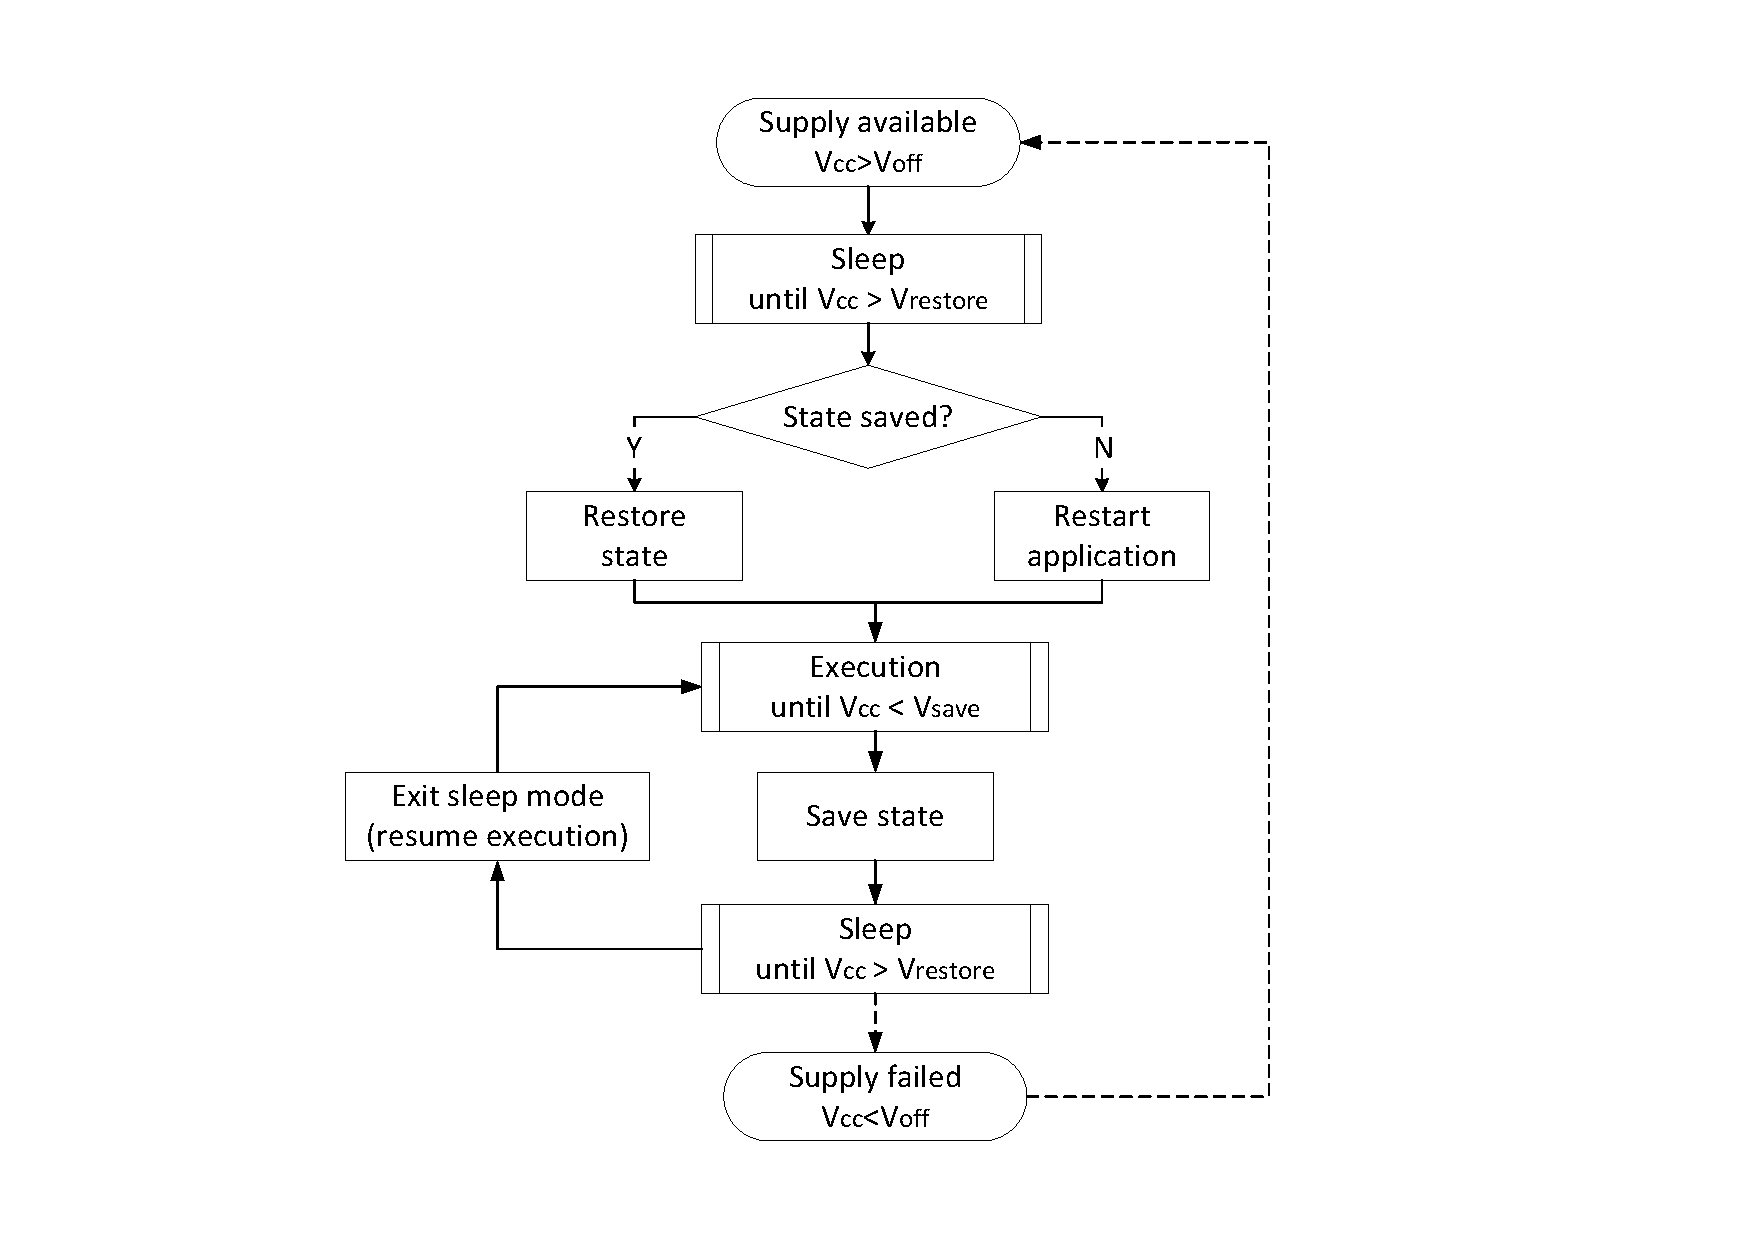
\includegraphics[width=12cm]{figure/work1/routine}
    \caption{System routine.}
    \label{Figure:routine}
\end{figure}

% platform
We refer to the measured data in published works \cite{6960060, 7403941} to model the load overheads. The data is acquired based on a TI MSP430FR5739 microcontroller running at 8 MHz. MSP430 series microcontrollers are a typical experimental platform in intermittent computing research because of its on-board NVM and low-power property. The energy storage capacity in this platform is 20\textmu F. We choose the power consumption of running 256-point complex Fast Fourier Transform (FFT) as the typical computing overhead. It is reported that MSP430 MCUs takes about 0.1 million cycles at 8 MHz to complete one 256-point FFT iteration \cite{fft}, so we set the cycle counts to deliver a result as 0.1 million cycles. The full parameter settings of the load model are listed in Table \ref{Table:overheads}. These parameter names represent the same meanings when used in the remaining part of this chapter.

\begin{table}[H]
    \caption{Parameter settings of the load model.}
    \label{Table:overheads}
    \centering
    \begin{tabular}{ccc}
    \toprule
    \textbf{Parameter} & \textbf{Value} & \textbf{Description}\\
    \midrule
    $V_{off}$ & 2.0 V & Minimum operating voltage \\
    $V_{save}$ & 2.2 V & Saving threshold \\
    $V_{restore}$ & 2.3 V & Restoring threshold \\
    $T_{save}$ & 1.40 ms & Saving time overhead \\
    $T_{restore}$ & 1.35 ms & Restoring time overhead \\
    $P_{save}$ &  2.13 mW & Saving power consumption \\
    $P_{restore}$ & 2.63 mW & Restoring power consumption \\
    $P_{exe}$ & 2.79 mW & Executing power consumption \\
    $P_{sleep}$ & 1.10 \textmu W & Sleeping power consumption \\ % reference
    % execution throughput rate, cycle counts to deliver a result
    \bottomrule
    \end{tabular}
\end{table}

%%%%%%%%%%%%%%%%%%%%%%%%%%%%%%%%%%%%%%%%%%
%%%%%%%%%%%%%%%%%%%%%%%%%%%%%%%%%%%%%%%%%%o

\section{Simulation Analysis} \label{Section:4}

Our simulation goals are two-fold: a) to explain the sizing effect of energy storage and energy harvester on intermittent computing performance, b) to demonstrate our sizing method. 

Section \ref{Section:4.1} explains the operating regions of intermittent computing devices given a range of power supply, which is useful for explanation in the following sections. Section \ref{Section:4.2} illustrates how the size of energy storage and energy harvesting has an impact on application performance of intermittent computing devices, and provides formulations to estimate the delivered performance. Section \ref{Section:4.3} and Section \ref{Section:4.4} respectively presents the sizing effects of energy storage and energy harvester under real-world deployment. Finally, Section \ref{Section:4.5} presents a combined sizing effect.

As the original energy storage capacity used in the previous intermittent computing works is 20\textmu F, this capacity is used as a baseline comparison for the following discussion of energy storage sizing.

\subsection{Operating Regions of Intermittent Computing Devices.} \label{Section:4.1}

% With only a limited amount of storage, 
Operating behaviours of intermittent computing devices can be divided into three regions according to application performance. As shown in Figure \ref{Figure:varyG}, an example simulation to demonstrate the three regions is done by measuring application throughput (FFT iterations) in one minute given minimum storage (20\textmu F) and constant irradiance at different levels. We denote the three regions by \textit{Off}, \textit{Switch}, and \textit{On}. These three regions are divided by the relationship between the harvested power and the system power consumption (including $P_{exe}$, $P_{sleep}$, and leakage power $P_{leak}$), which is affected by energy conditions at run time. 

\begin{figure}[H]
    \centering
    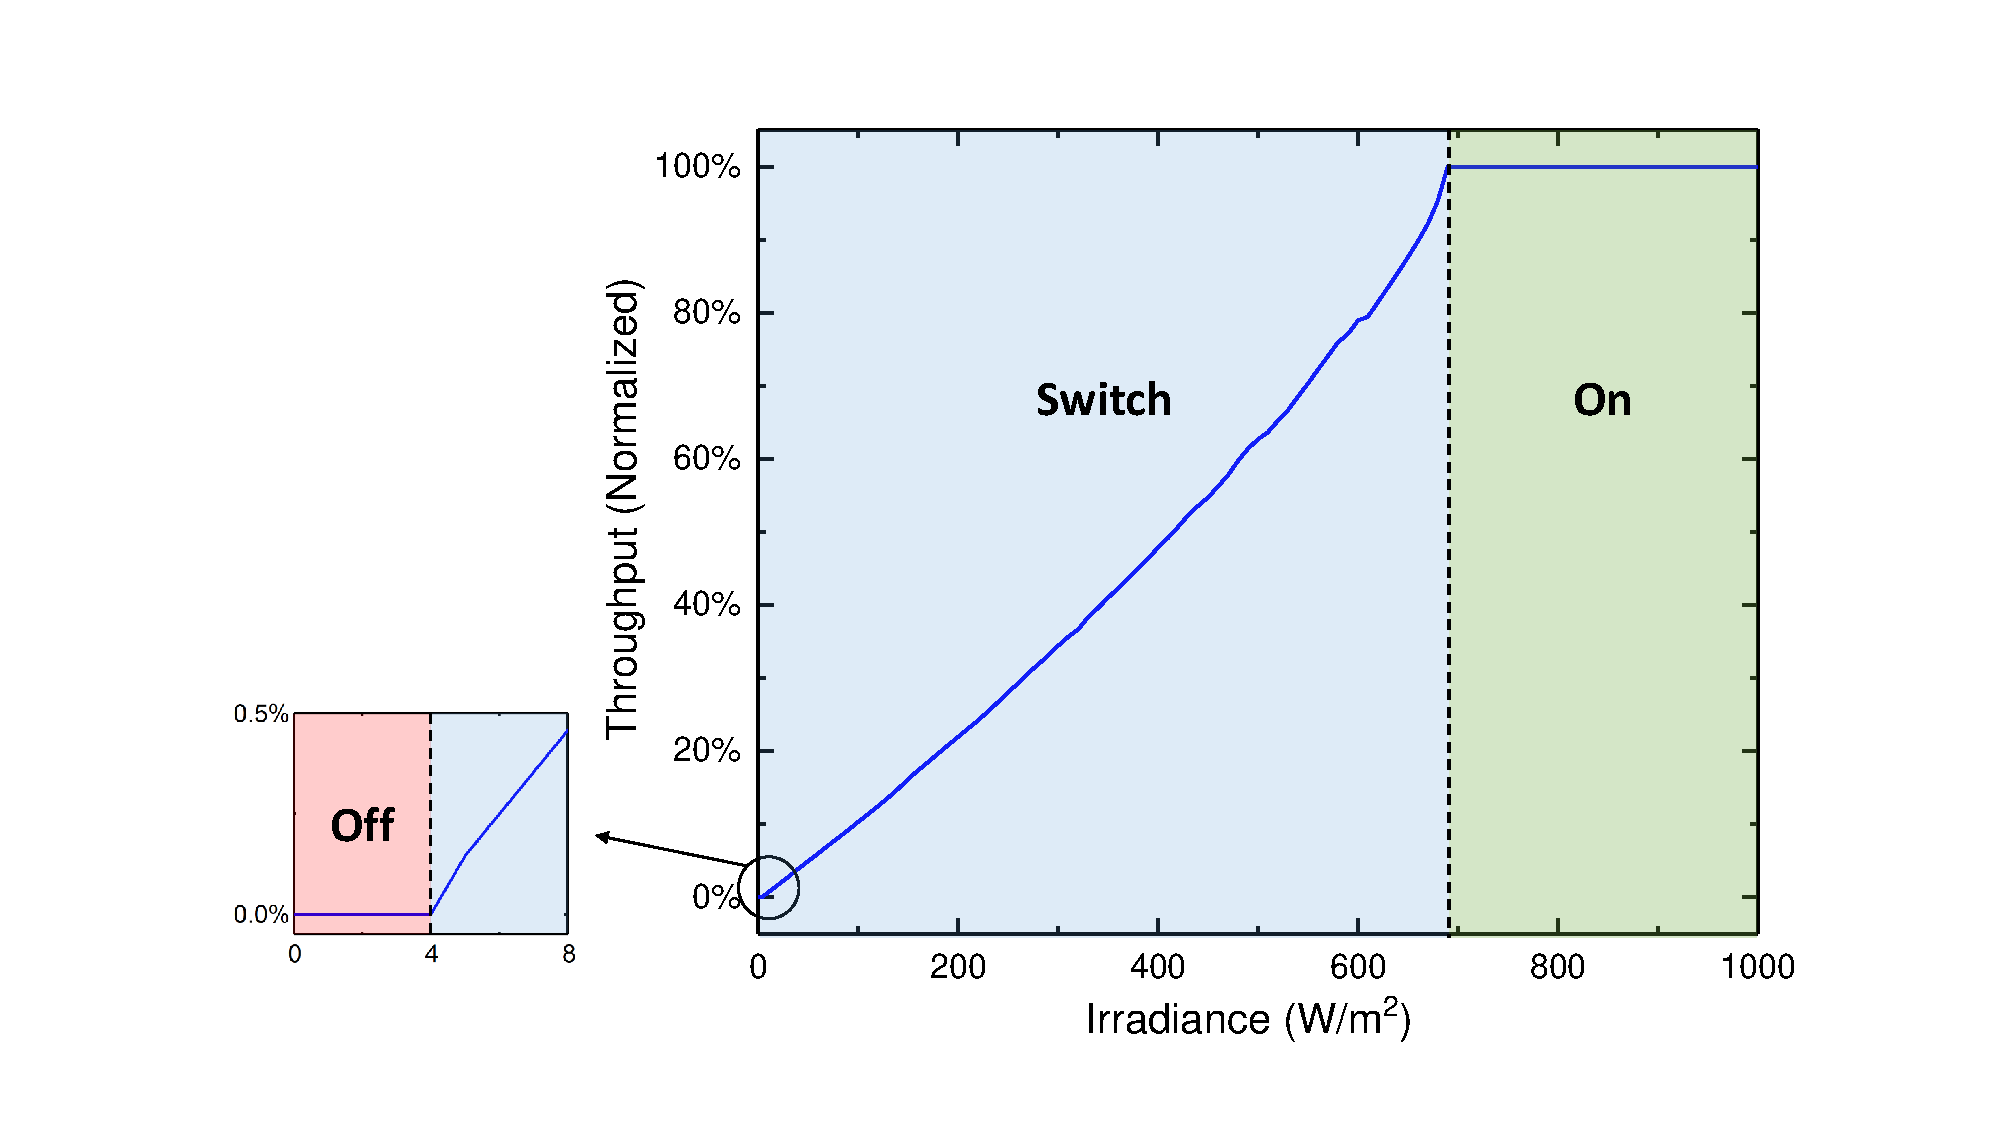
\includegraphics[width=12cm]{figure/work1/varyG}
    \caption{Three operating regions given irradiance at different intensities (performance indicated by normalized FFT throughput given 20\textmu F capacitance and 1-min constant irradiance).}
    \label{Figure:varyG}
\end{figure}

\textit{Off}: When $P_{harvest} < P_{sleep} + P_{leak}$, the device cannot wake up. The supply voltage $V_{cc}$ cannot be charged above the restore threshold $V_{restore}$ to start execution. Here, $P_{sleep}$ is induced after $V_{cc}$ goes above the minimum operating voltage $V_{off}$ and the device waits for $V_{cc}$ to reach $V_{restore}$ (when $V_{off} < V_{cc} < V_{restore}$). 

\textit{Switch}: When $P_{sleep} + P_{leak} < P_{harvest} < P_{exe} + P_{leak}$, the device executes intermittently. $V_{cc}$ can be charged up to trigger execution as $P_{harvest} < P_{sleep} + P_{leak}$. However, as $P_{harvest} < P_{exe} + P_{leak}$, the energy in energy storage needs to compensate for this power difference, causing $V_{cc}$ to drop below $V_{save}$, where the device saves its state and enters sleep mode. The device sleeps until $V_{cc}$ charges to $V_{restore}$ again and then resumes the execution. In this region, $V_{cc}$ oscillates between $V_{restore}$ and $V_{save}$, "switching" on and off the execution. Generally, in this operating region, higher $P_{harvest}$ leads to higher application performance (i.e. completed iterations in a unit of time).

\textit{On}: When $P_{harvest} > P_{exe} + P_{leak}$, the device execute constantly as the supply voltage $V_{cc}$ never fails. The excessive power is dissipated through circuitry, or overcharges $V_{cc}$ which affects harvesting efficiency and reduces $P_{harvest}$ to the power consumption level. In this model case, charging $V_{cc}$ above the maximum power point of the PV cell reduces $P_{harvest}$, and $V_{cc}$ is stable when $P_{harvest} = P_{exe} + P_{leak}$. 

% \begin{table}[H]
%     \caption{Operating Regions.}
%     \label{Table:overheads}
%     \centering
%     \begin{tabular}{ccc}
%     \toprule
%     \textbf{Region} & \textbf{Condition} & \textbf{Feature}\\
%     \midrule
%     OFF & $I_{harvest} < I_{sleep} + I_{leak}$ & Never execute \\
%     \bottomrule
%     \end{tabular}
% \end{table}

\subsection{Sizing Effect of Energy Storage and Energy Harvester on Performance} \label{Section:4.2}

As shown in Figure \ref{Figure:VaryCapThrp}, the effect of energy storage capacity on application performance is explored by increasing capacitance from 20\textmu F (the baseline storage) to 200\textmu F under four levels of constant irradiance. This preliminary result shows that increasing capacitance (to around 80\textmu F) leads to performance improvement for those harvesting power conditions in the Switch region (e.g. 200$W/m^2$, 400$W/m^2$, 600$W/m^2$ irradiance), but does not make benefit in the On region (e.g. 800$W/m^2$). However, this improvement in the Switch region is offset by larger capacitor leakage if adding too much capacitance (e.g. over 200\textmu F). Also, the maximum performance improvement gained from sizing storage reduces as the energy source gets more intense (from 200 to 800 $W/m^2$).

\begin{figure}[H]
    \centering
    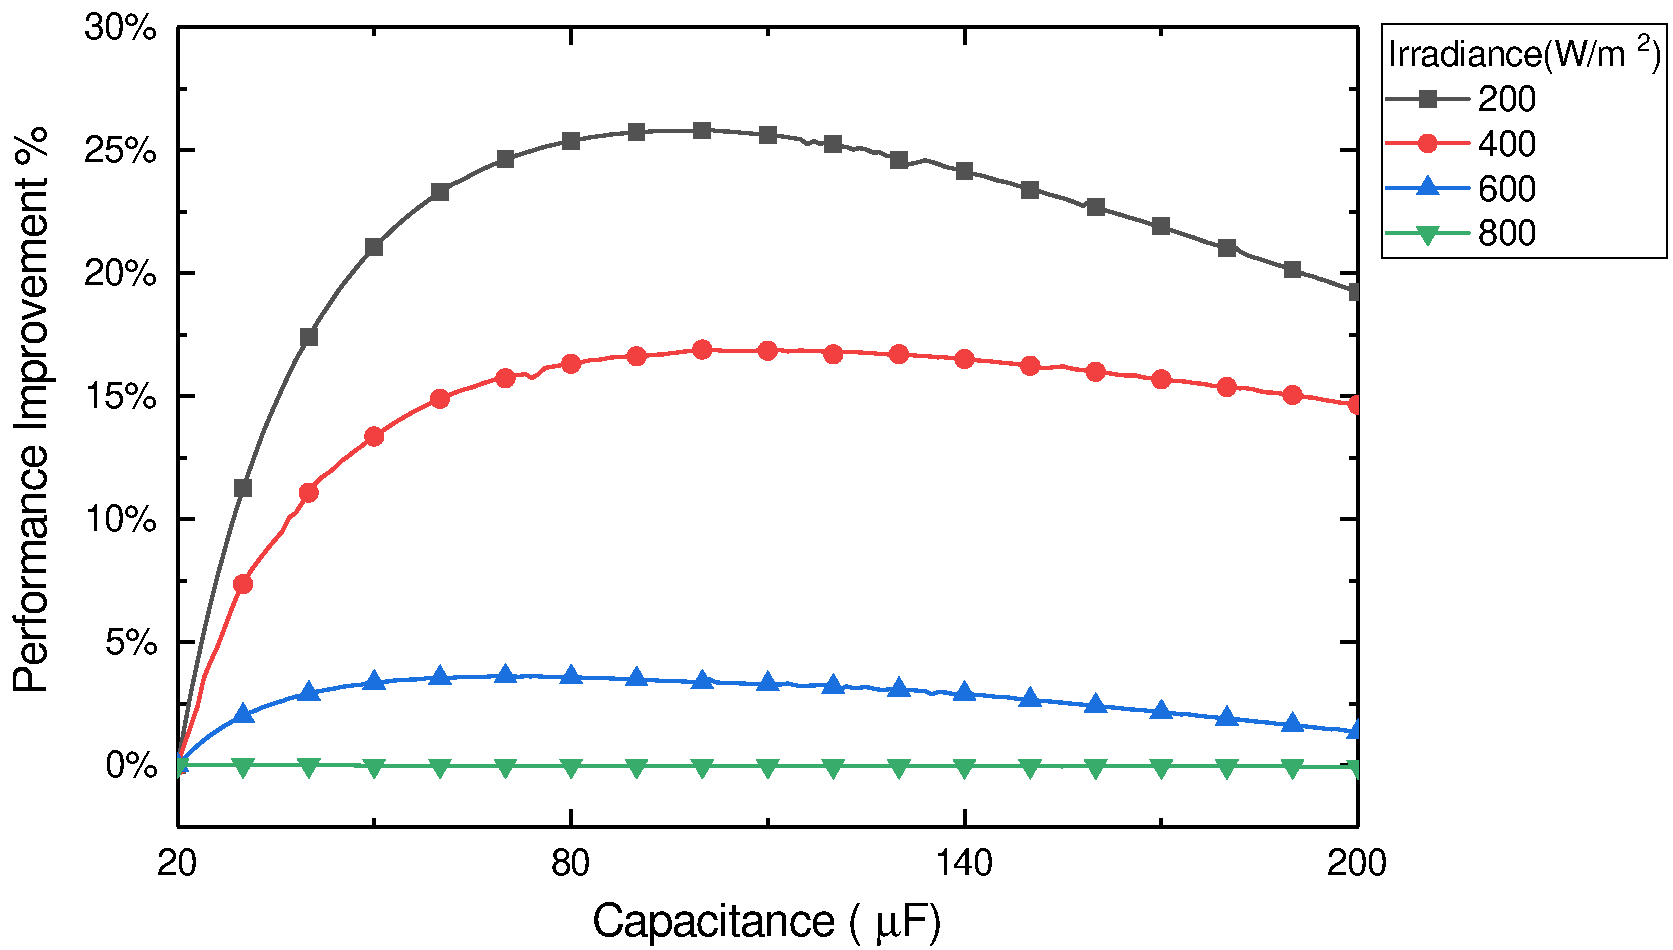
\includegraphics[width=13cm]{figure/work1/VaryCapThrp}
    \caption{Performance improvement (application throughput improvement compared to 20\textmu F capacitance at each energy condition) by increasing capacitance from 20\textmu F to 200\textmu F (at 1\textmu F resolution) given four levels of constant irradiance. }
    \label{Figure:VaryCapThrp}
\end{figure}

To further explain this effect, we investigate a segment of the supply voltage $V_{cc}$ traces at 20\textmu F (minimum performance) and 100\textmu F (maximum performance) under 400$W/m^2$ irradiance (an energy source condition in the Switch region). As shown in Figure \ref{Figure:Vcctrace}, in both traces, $V_{cc}$ experiences discharging and charging intervals periodically. The discharging interval includes resuming execution at $V_{restore}$ = 2.3V and saving state at $V_{save}$ = 2.2V (here, this platform does not need to restore state to resume execution after it wakes up from the sleep mode because this platform keeps volatile state in the sleep mode). In this test, these discharging and charging intervals are periodic because the applied irradiance is constant in these tests. Comparing the 100\textmu F trace to the 20\textmu F one, the increased capacitance prolongs the discharging and charging period, so the save and restore operations are less frequent. The reduction of save and restore operations spares more energy on execution, resulting in higher application throughput. However, increasing capacitance also causes higher leakage, which reduces the amount of usable energy and offsets the improvement gained from increasing storage. This trade-off should be evaluated to find the optimal storage size for maximising performance. 
% starts discharging when reaching the restore threshold ($V_{restore}$ = 2.3V) and triggers saving operation when dropping to the save threshold ($V_{save}$ = 2.2V)

\begin{figure}[H]
    \centering
    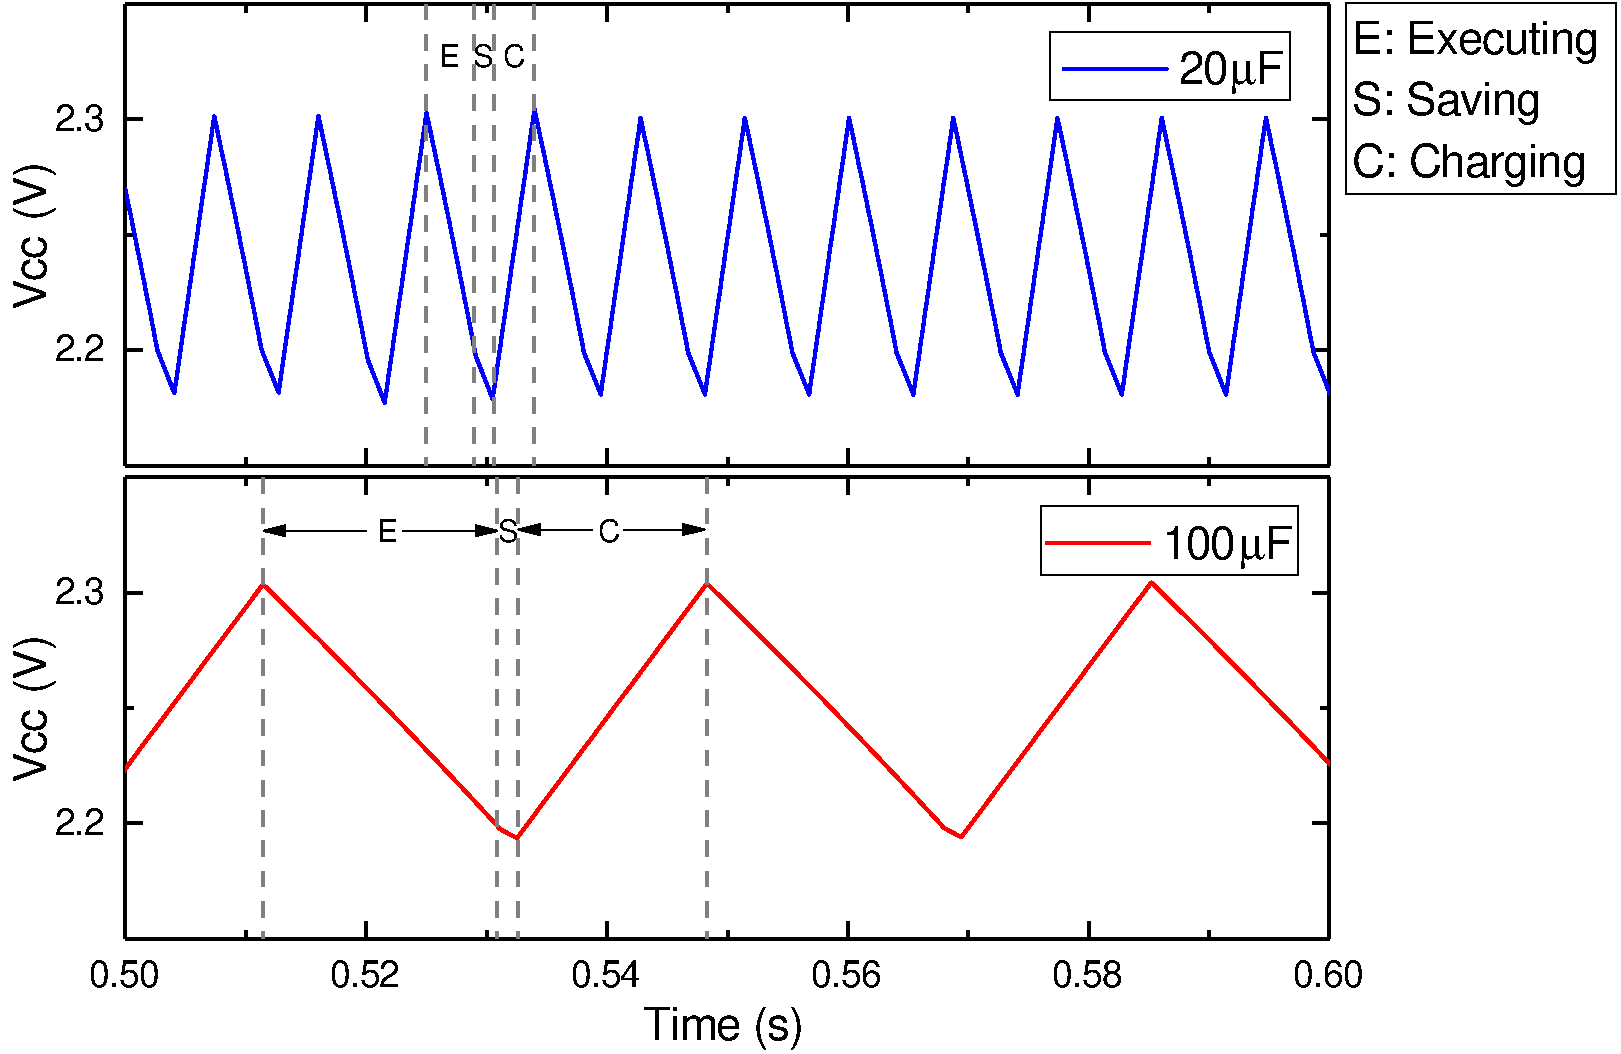
\includegraphics[width=13cm]{figure/work1/Vcctrace05-06}
    \caption{Supply Voltage $V_{cc}$ trace segments at 20\textmu F and 100\textmu F under 400$W/m^2$ constant irradiance.}
    \label{Figure:Vcctrace}
\end{figure}

Mathematical equations are developed to abstract this system behaviour and numerically find the trade-off in sizing storage. For covering general cases, a restore operation is included in this analysis between waking up from the sleep mode and resuming execution. 

In one period, the device goes through charging, restoring, executing, and saving intervals sequentially. If we denote $V_{postrestore}$ and $V_{postsave}$ as the voltage after restoring and saving operations, $V_{postrestore}$ and $V_{postsave}$ can be calculated as:

\begin{equation}
    V_{postsave} = V_{save} + \frac{(I_{harvest} - I_{leak} - I_{save}) T_{save}}{C}
    \label{Equation:Vpostsave}
\end{equation}

\begin{equation}
    V_{postrestore} = V_{restore} + \frac{(I_{harvest} - I_{leak} - I_{restore}) T_{restore}}{C}
    \label{Equation:Vpostrestore}
\end{equation}

where $I_{harvest}$, $I_{save}$, and $I_{restore}$ are the average current of harvesting, saving, and restoring in these intervals. If we denote $I_{exe}$ as the average current consumption of execution, the time spent on useful execution $T_{exe}$ can be expressed as:

\begin{equation}
    T_{exe} = \frac{C(V_{postrestore} - V_{save})}{I_{exe} + I_{leak} - I_{harvest}}
    \label{Equation:texe}
\end{equation}

Then, the charging and discharging intervals can be described as:

\begin{equation}
    T_{charge} = \frac{C(V_{restore} - V_{postsave})}{I_{harvest} - I_{leak} - I_{sleep}}
    \label{Equation:tcharge}
\end{equation}

\begin{equation}
    T_{discharge} = T_{restore} + T_{exe} + T_{save}
    \label{Equation:tdischarge}
\end{equation}

Combining Equation \ref{Equation:texe}, \ref{Equation:tcharge}, and \ref{Equation:tdischarge}, we can obtain the percentage of time spent on useful execution:

\begin{equation}
    T_{exe\%} = \frac{T_{exe}}{T_{charge} + T_{discharge}}
\end{equation}

Therefore, the average performance $\overline{S_{app}}$ (represented by application throughput per second) given a constant harvested current in the Switch region can be approximated as:

\begin{equation}
    \overline{S_{app}} = T_{exe\%}\frac{f_{CPU}}{N_{appcycles}}
\end{equation}

where $f_{CPU}$ is the CPU clock frequency, and $N_{appcycles}$ is the number of cycles to complete an application iteration. Here, $\overline{S_{app}}$ can be translated to a function of $C$ and $I_{harvest}$ in the Switch region because all of other parameters are known in parameter settings. After applying the conditions for the Off and On regions (Off: $P_{harvest} < P_{sleep} + P_{leak}$, On: $P_{harvest} > P_{exe} + P_{leak}$), this function for all energy source conditions becomes:

\begin{equation}
    \overline{S_{app}} = f(C, I_{harvest}) = \left\{\begin{aligned}
        & 0 & , & \quad Off \\
        & T_{exe\%} (C, I_{harvest}) \frac{f_{CPU}}{N_{appcycles}} & , & \quad Switch \\
        & \frac{f_{CPU}}{N_{appcycles}} & , & \quad On
    \end{aligned}
    \right.
    \label{Equation:paverage}
\end{equation}

In Equation \ref{Equation:paverage}, we get the relationship between the application performance and the size of energy harvester and storage. $C$ represents the size of the energy storage. $I_{harvest}$ is determined by the energy source condition and the size of the energy harvester. 

We evaluate this theoretical average performance $\overline{S_{app}}$ with our simulation results. An average operating voltage is assumed at $(V_{save} + V_{restore})/2$ to calculate $I_{harvest}$, $I_{exe}$, $I_{sleep}$, $I_{save}$, and $I_{restore}$ in the Switch region. As shown in Figure \ref{Figure:veriTheory}, the theoretical $\overline{S_{app}}$ is compared with simulated $\overline{S_{app}}$ at three energy conditions. The overall mean absolute percentage error (MAPE) is 0.316\%. Therefore, these equations explain the simulation results on performance changes by increasing storage in Figure \ref{Figure:VaryCapThrp}. These equations for estimating the application performance $\overline{S_{app}}$ given constant energy conditions will be used later to estimate $\overline{S_{app}}$ in variable energy conditions. 

% your equations explain what roughly happen in the model/simulation. 
% \dots what does this equation indicate? what cause the change in sizing storage?
% \dots applicable cases. reactive.

\begin{figure}[H]
    \centering
    \begin{subfigure}{0.325\textwidth}
        \centering
        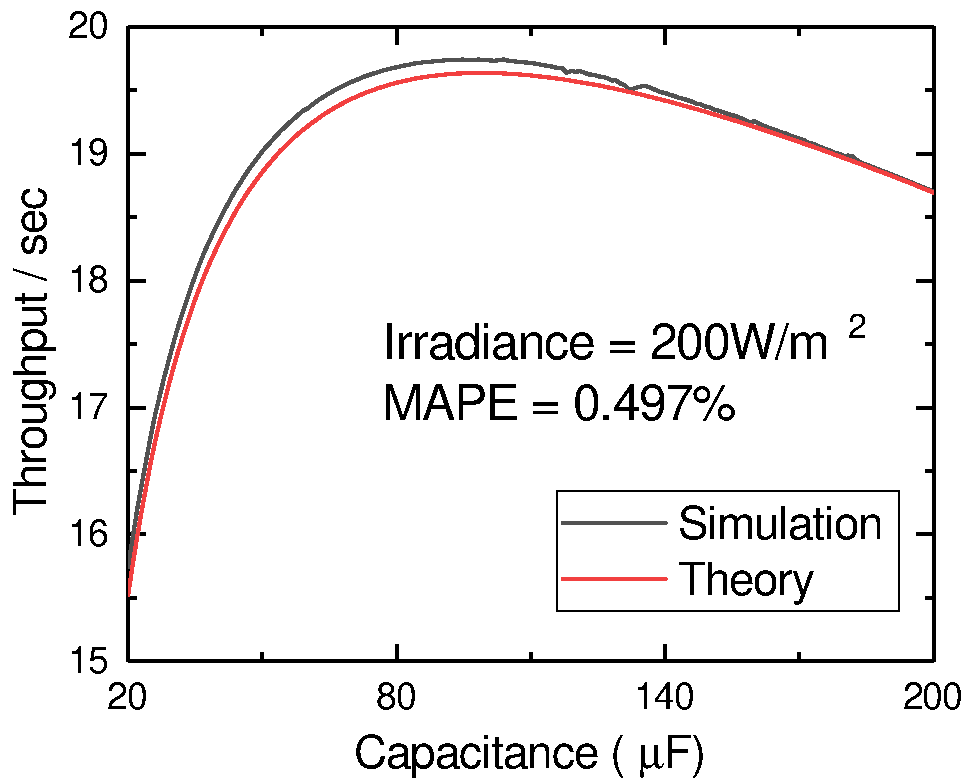
\includegraphics[width=\textwidth]{figure/work1/veriTheory200}
        \caption{Irradiance = 200 $W/m^2$}
    \end{subfigure}
    \begin{subfigure}{0.325\textwidth}
        \centering
        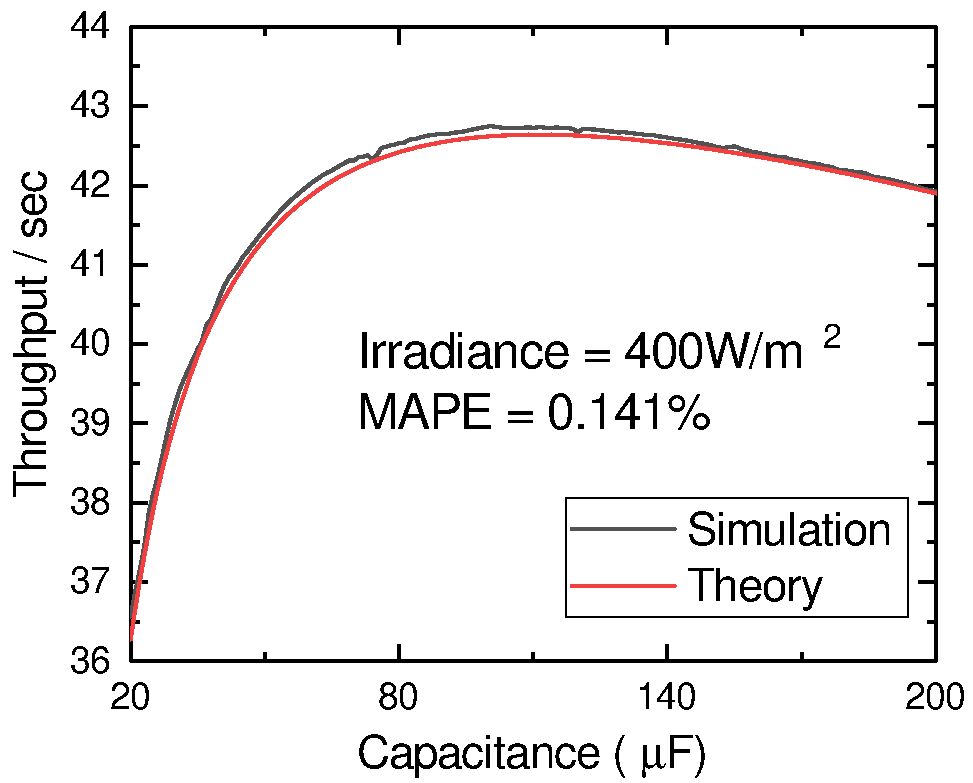
\includegraphics[width=\textwidth]{figure/work1/veriTheory400}
        \caption{Irradiance = 400 $W/m^2$}
    \end{subfigure}
    \begin{subfigure}{0.325\textwidth}
        \centering
        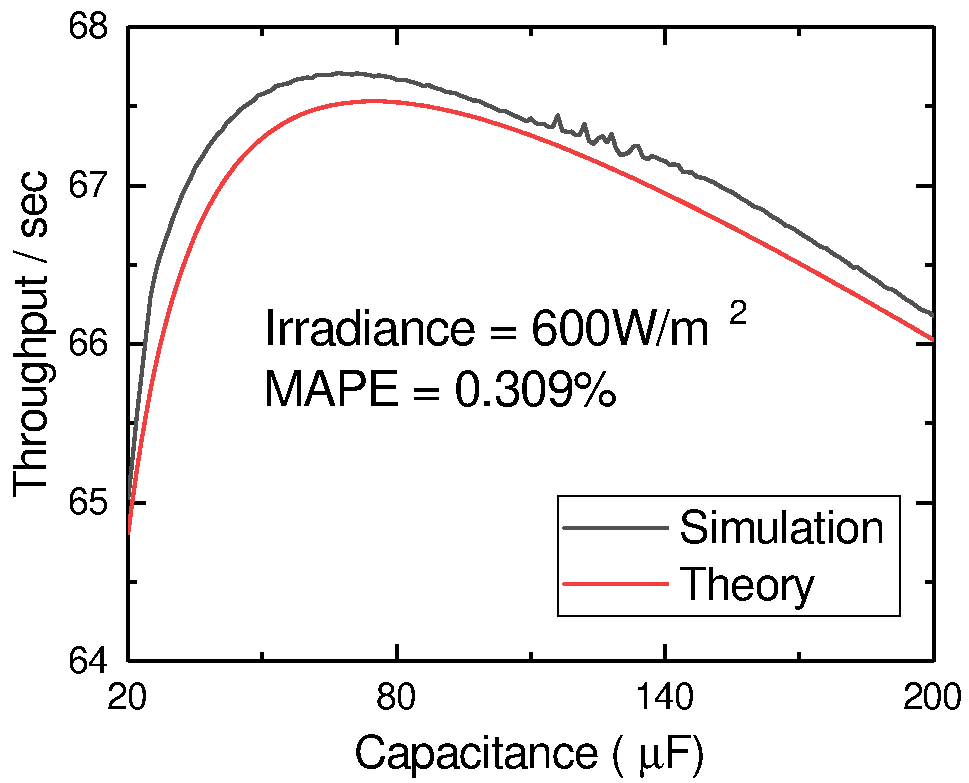
\includegraphics[width=\textwidth]{figure/work1/veriTheory600}
        \caption{Irradiance = 600 $W/m^2$}
    \end{subfigure}
       \caption{Comparison between estimated performance using formulations and simulated performance under constant irradiance.}
       \label{Figure:veriTheory}
\end{figure}

The above analysis indicates that the performance improvement by using larger energy storage is due to reduced saving and restoring overheads in the Switch region, which leads to increased effective computing energy. However, increasing storage also leads to higher leakage consumption. This trade-off is theoretically analysed with mathematical relationships. 

\subsection{Sizing Energy Storage under Real-World Irradiance Conditions} \label{Section:4.3}

We further apply this estimating method for sizing energy storage given real-world energy conditions. 

Real-world energy conditions are time-varying and may cover three operating regions. The previous equations can adapt to time-varying energy conditions by sorting variable energy conditions into time lengths spent on each level of energy condition. To demonstrate this, our method analyses the time distribution of real-world irradiance data, calculates the corresponding performance at each irradiance, and integrate them with time to obtain total throughput (or average performance).

This method is compared with time-based simulation results given monthly irradiance in four different seasons (different amounts of energy sources). As shown in Figure \ref{Figure:CapSizeReal}, an average MAPE is given by 0.892\%. All the four tests shows a maximum performance around 80\textmu F. Comparing the performance at 80\textmu F capacitance to the 20\textmu F one, the performance improvement in the listed tests is 14.5\%, 5.4\%, 4.5\%, and 8.7\% respectively, with an average improvement of 8.3\%.

% \dots how much is the reduction of saving and restoring overhead?

\begin{figure}[H]
    \centering
    \begin{subfigure}{0.49\textwidth}
        \centering
        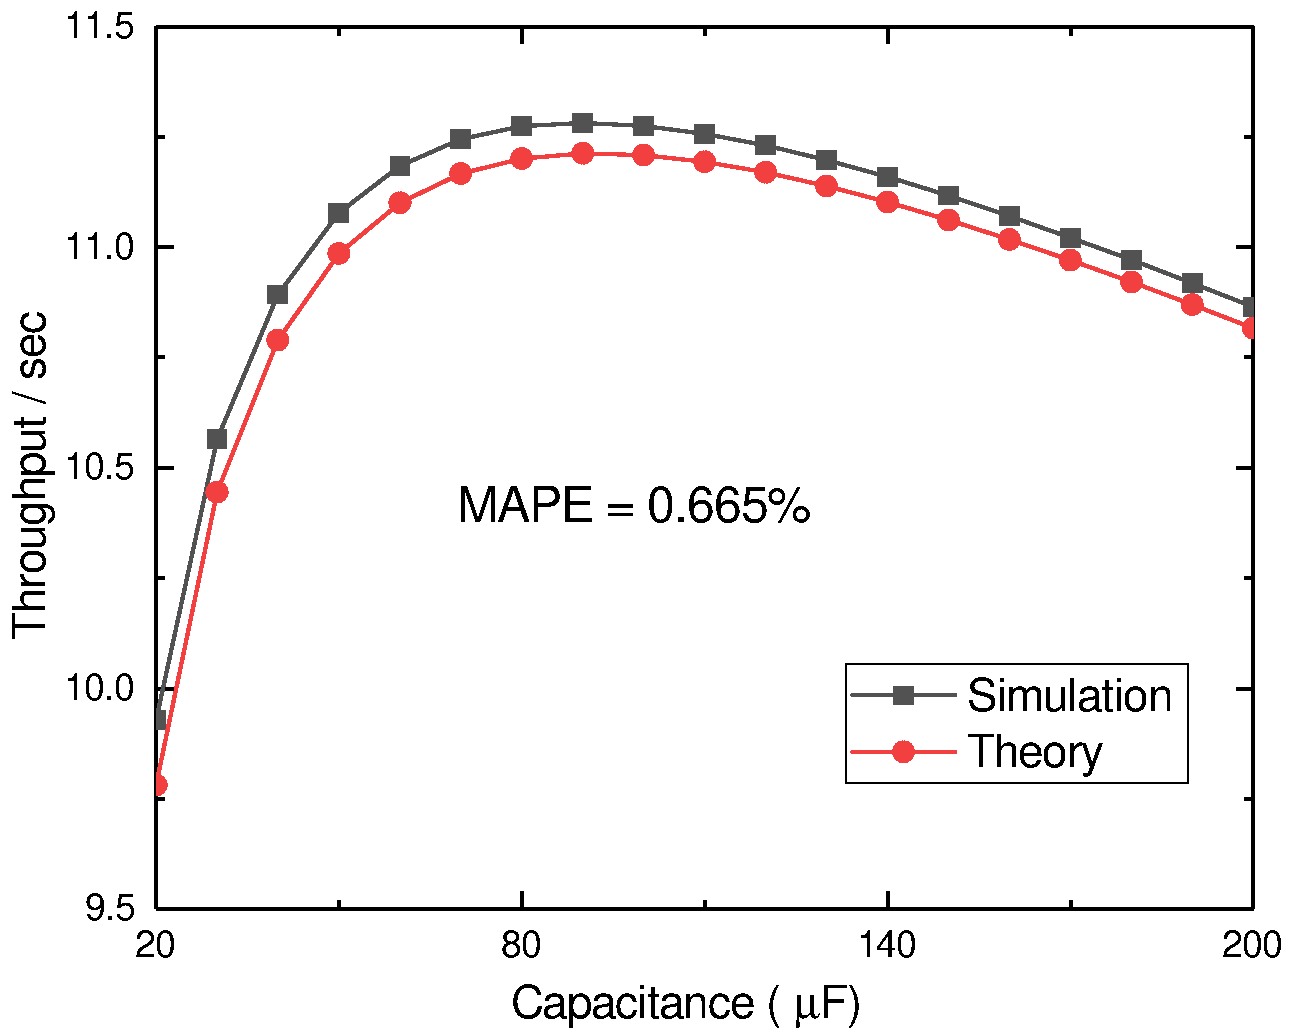
\includegraphics[width=\textwidth]{figure/work1/CapDenvJan}
        \caption{Jan 2018, Denver}
    \end{subfigure}
    \begin{subfigure}{0.49\textwidth}
        \centering
        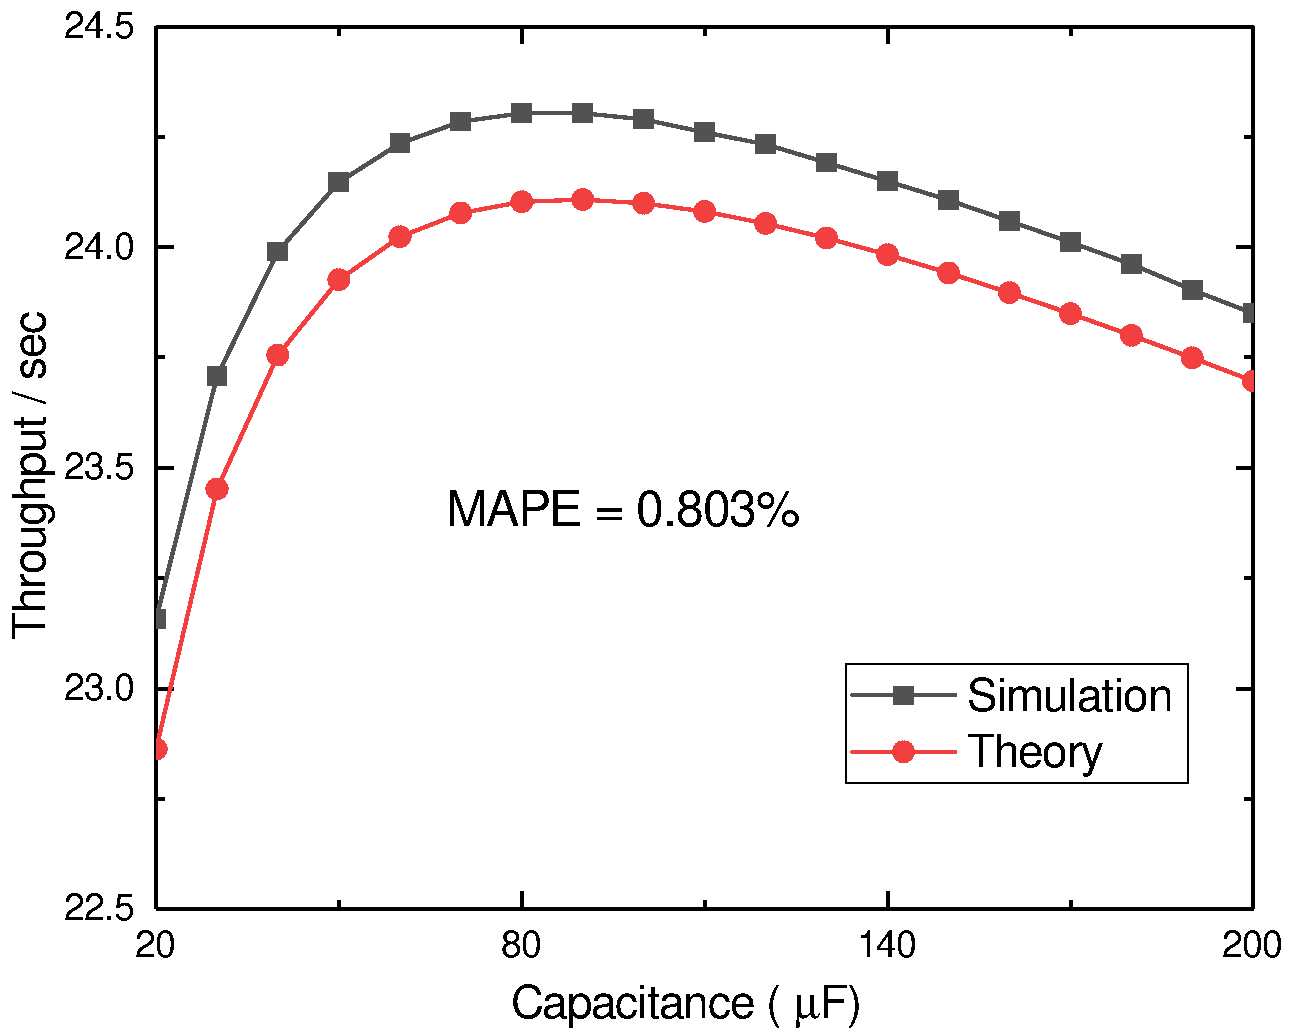
\includegraphics[width=\textwidth]{figure/work1/CapDenvApr}
        \caption{Apr 2018, Denver}
    \end{subfigure}
    \par\bigskip
    \begin{subfigure}{0.49\textwidth}
        \centering
        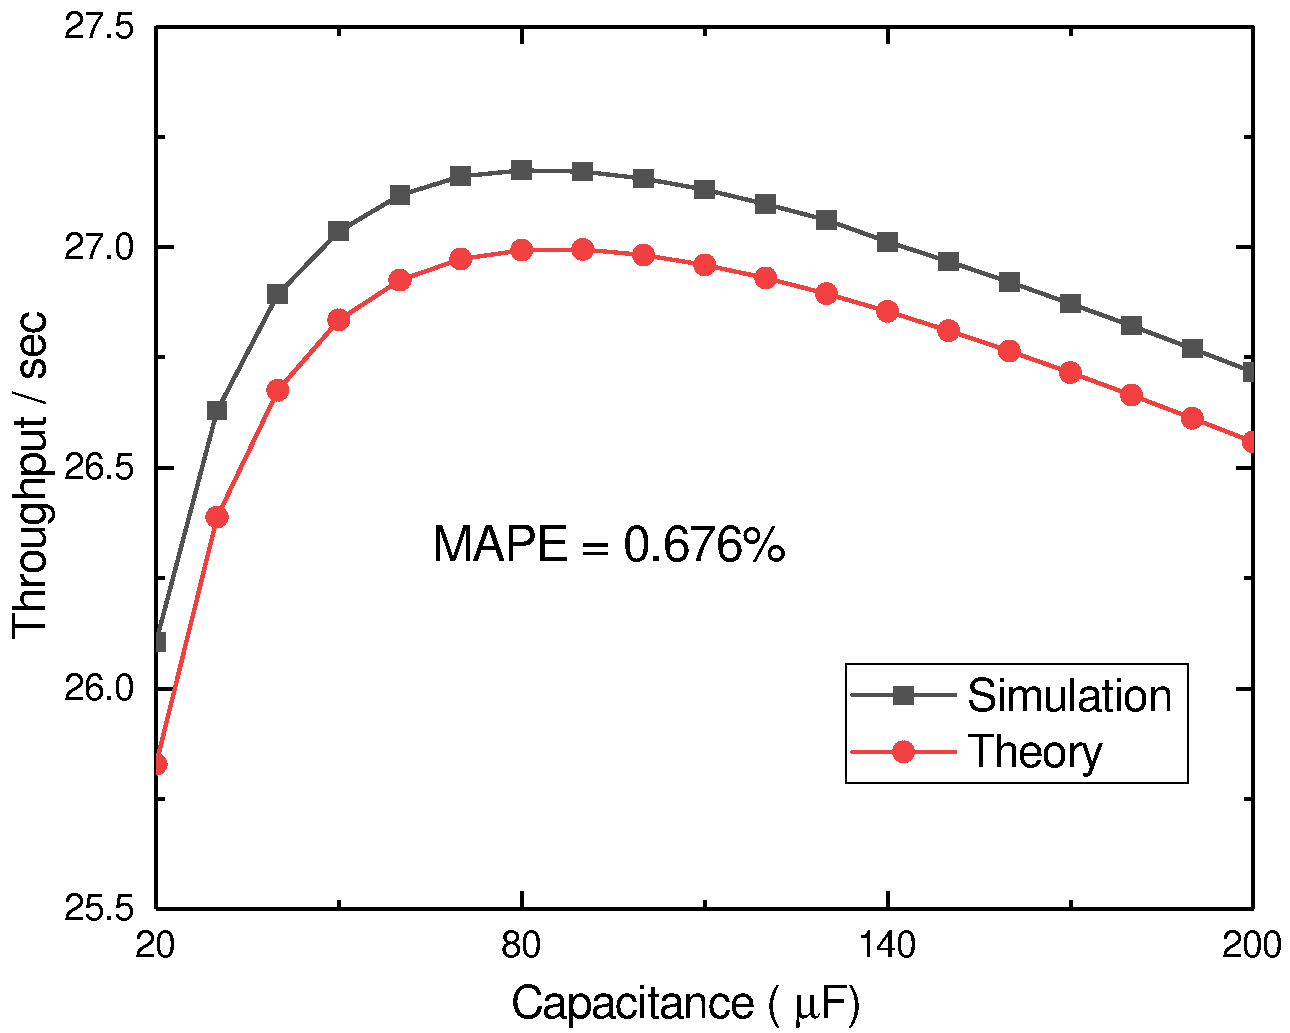
\includegraphics[width=\textwidth]{figure/work1/CapDenvJul}
        \caption{Jul 2018, Denver}
    \end{subfigure}
    \begin{subfigure}{0.49\textwidth}
        \centering
        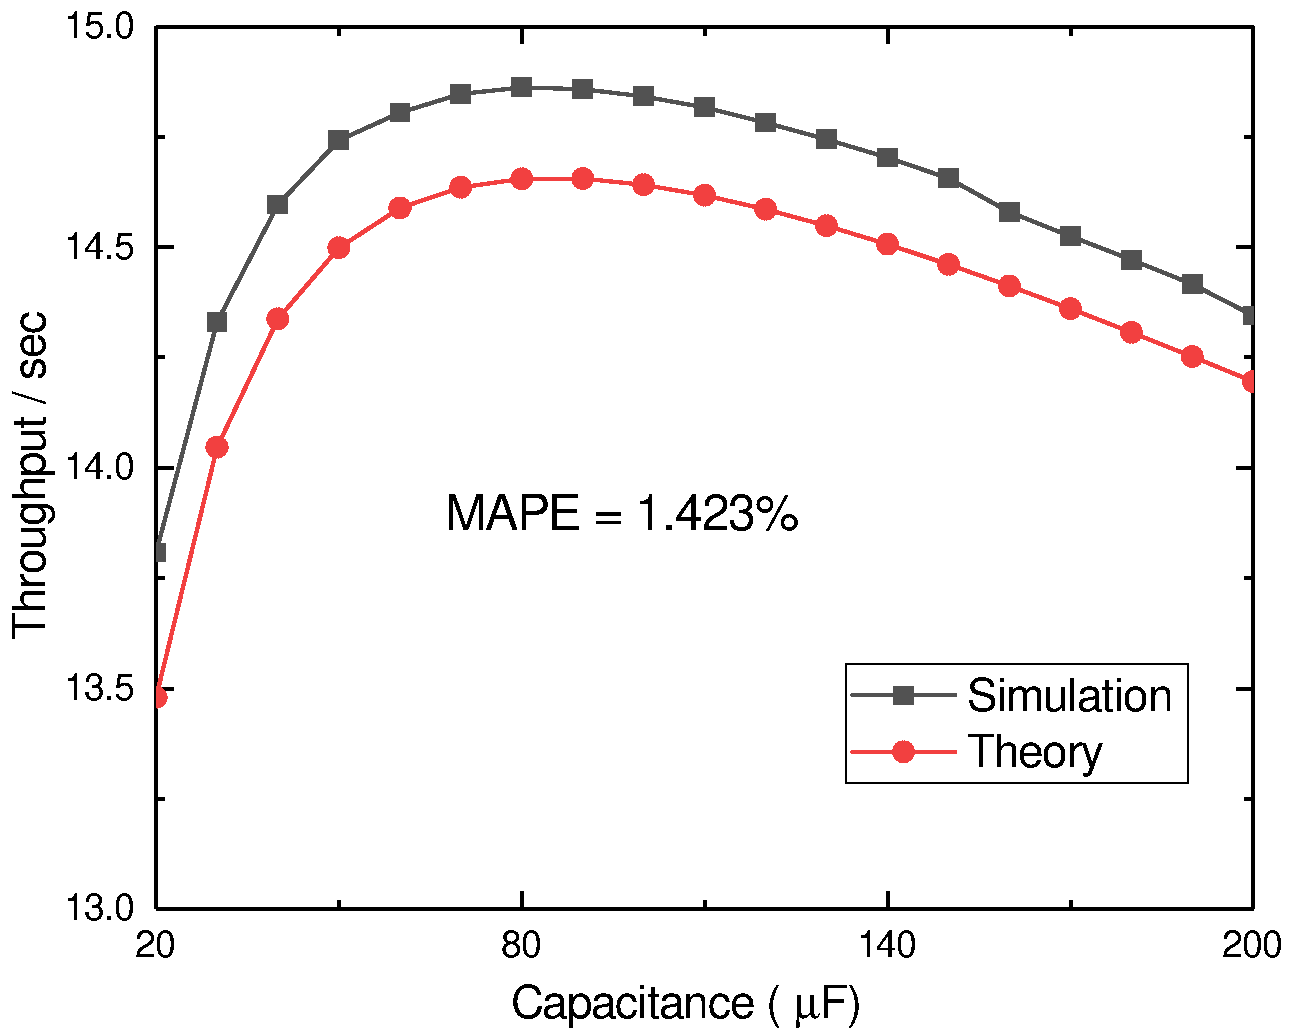
\includegraphics[width=\textwidth]{figure/work1/CapDenvOct}
        \caption{Oct 2018, Denver}
    \end{subfigure}
    \caption{Comparison between estimated and simulated average performance under real-world irradiance data.}
    \label{Figure:CapSizeReal}
\end{figure}
% errors, hysteresis changing between Switch and On

We apply this method to estimate the sizing effect of energy storage on an annual time scale. As shown in Figure \ref{Figure:year2018}, increasing storage from 20\textmu F to 80\textmu F improves the overall throughput by 6.7\% and 5.4\% at the two example locations respectively (given the harvester size used in the prior simulations). However, the system operates in the On region for 10.8\% and 14.6\% of time respectively, which indicates there is excessive power to use. Increasing energy storage cannot make benefit on throughput in the On region, so if the energy conditions are poorer or the harvester size is smaller (where the system spends more time in the Switch region) sizing energy storage will make more improvement. 

\begin{figure}[H]
    \centering
    \begin{subfigure}{0.49\textwidth}
        \centering
        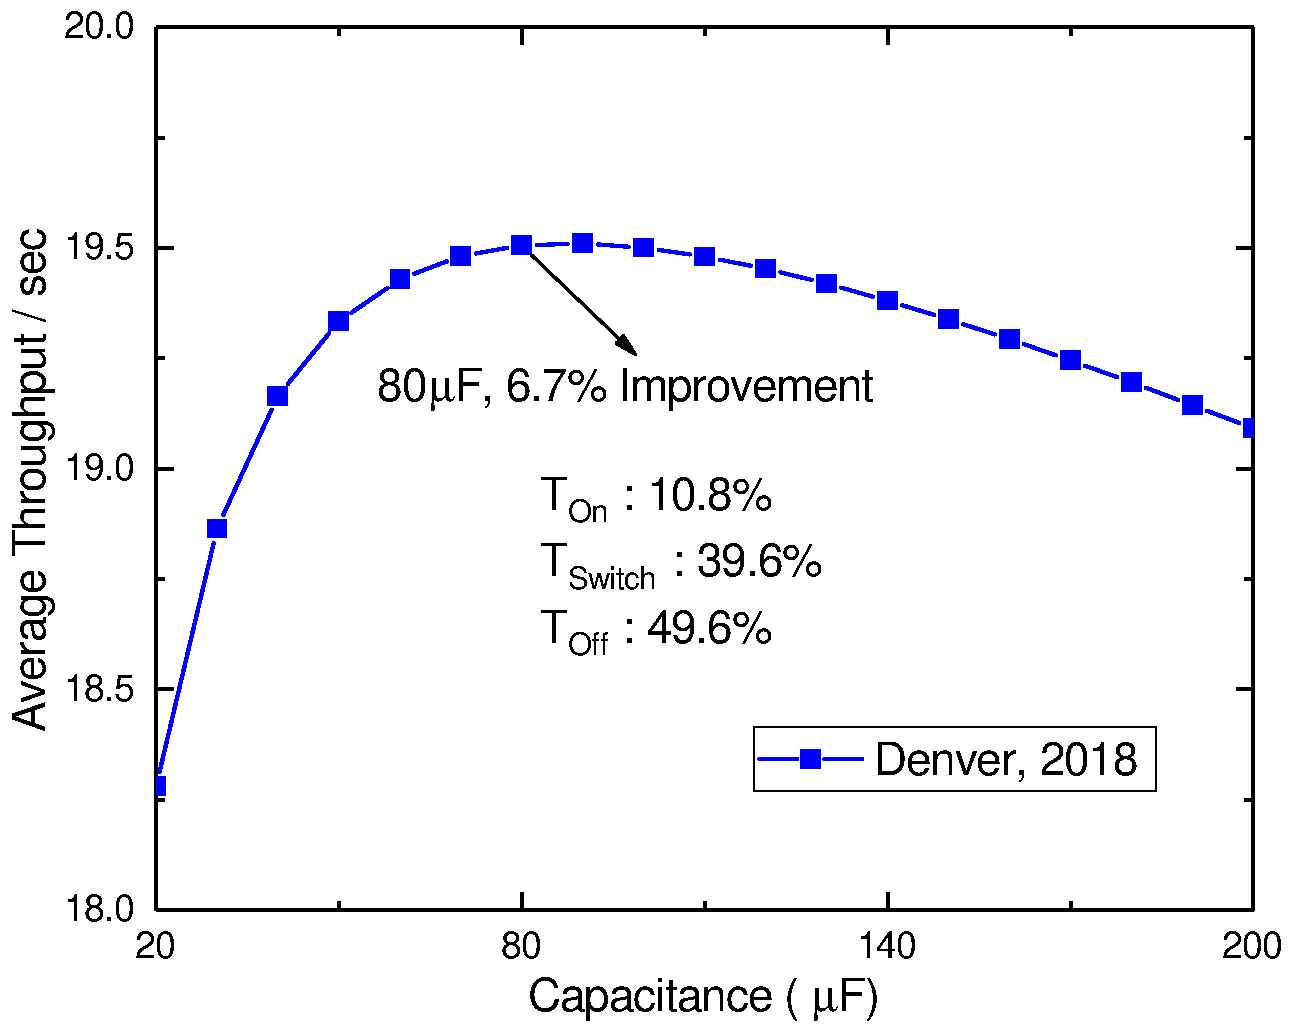
\includegraphics[width=\textwidth]{figure/work1/denver2018}
        \caption{Denver, 2018}
    \end{subfigure}
    \begin{subfigure}{0.49\textwidth}
        \centering
        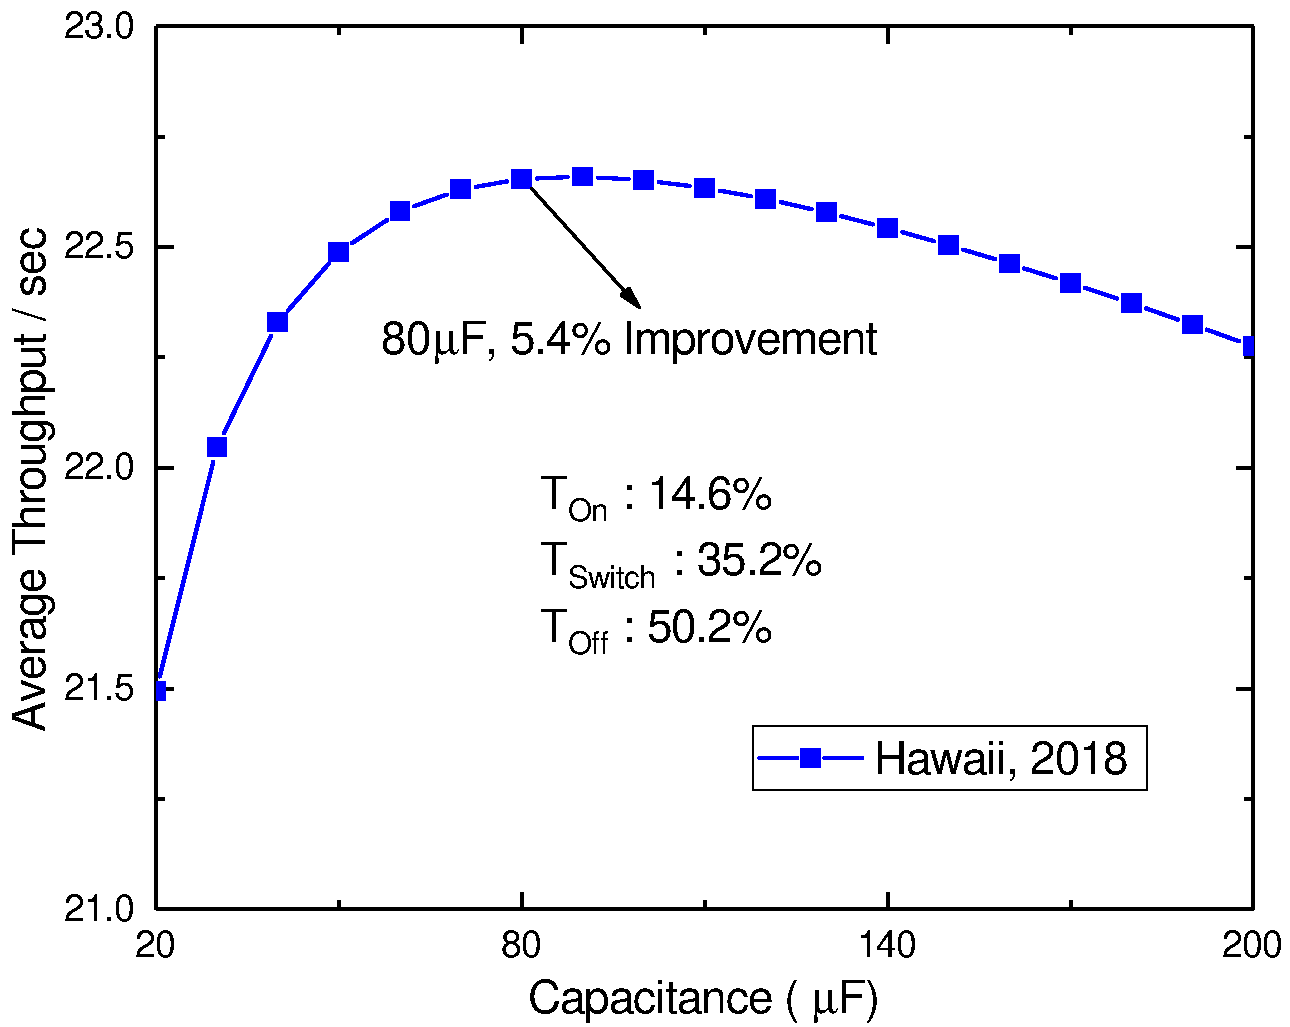
\includegraphics[width=\textwidth]{figure/work1/hawaii2018}
        \caption{Hawaii, 2018}
    \end{subfigure}
    \caption{Performance estimation given annual solar data, with the time ratio spent on each operating region denoted as $T_{On}$, $T_{Switch}$, and $T_{Off}$.}
    \label{Figure:year2018}
\end{figure}

The dimensions of capacitors varies with its capacity. This capacity-dimension relationship of capacitors is non-linear and largely depends on the packaging methods. A reference for capacitance (in the range discussed) and corresponding dimensions of three example commercial capacitors is listed in Table \ref{Table:capdimension}. Comparing the suggested 80\textmu F capacitor to the minimum 20\textmu F capacitance, which corresponds to 22\textmu F and 82\textmu F capacitors as the nearest available ones in the datasheet of aluminum capacitors, adding this amount of capacitance does not increase the actual dimensions.

\begin{table}[H]
    \caption{Actual dimensions of commercial aluminum and tantalum capacitors with capacitance in the discussed range and 10V rated voltage (D: diameter, L: length, W: width, H: height, unit: millimeters).}
    \label{Table:capdimension}
    \centering
    \begin{tabular}{cccc}
    \toprule
    \textbf{Capacitance} & \textbf{Aluminum} \cite{alcapacitor} & \textbf{Tantalum (Surface Mount)} \cite{tacap1} & \textbf{Tantalum (Dipped Radial Leaded)} \cite{tacap2} \\
    \midrule
    22\textmu F & D5$\times$L11 & L3.2$\times$W1.6$\times$H1.6 & D5.5$\times$L10.5 \\
    33\textmu F & D5$\times$L11 & L3.5$\times$W2.8$\times$H1.9 & D6.0$\times$L11.5 \\
    47\textmu F & D5$\times$L11 & L3.5$\times$W2.8$\times$H1.9 & D6.5$\times$L11.5 \\
    68\textmu F & N/A           & L3.5$\times$W2.8$\times$H1.9 & D7.0$\times$L12.0 \\
    82\textmu F & D5$\times$L11 & N/A                          & N/A \\
    100\textmu F & D5$\times$L11 & L3.5$\times$W2.8$\times$H1.9 & D8.5$\times$L14.0 \\
    120\textmu F & N/A           & L7.3$\times$W4.3$\times$H4.0 & N/A \\
    150\textmu F & D6.3$\times$L11 & L6.0$\times$W3.2$\times$H2.5 & D9.0$\times$L16.0 \\
    220\textmu F & D6.3$\times$L11 & L7.3$\times$W4.3$\times$H2.8 & D10.0$\times$L17.0 \\
    \bottomrule
    \end{tabular}
\end{table}

\subsection{Sizing Energy Harvester under Real-World Irradiance Conditions} \label{Section:4.4}

After exploring the effect of sizing energy storage, we move to explore the effect of sizing energy harvester. Clearly, enlarging energy harvester size, i.e. PV panel area in this case, increases the total amount of harvesting energy, and hence, increases the total application throughput. However, given a certain load deployed under real-world energy conditions, an over-provisioned energy harvester provides more power than the system consumes most of the time. At this point, increasing harvester size makes insignificant improvement on throughput. To evaluate an efficient energy harvester size, we introduce the ratio of the average performance to the energy harvester size (P/S ratio) as a measurement. This measurement indicates how efficiently the harvester size contributes to the application throughput. In our example system powered by PV cells, this measurement corresponds to performance per unit area of PV cells. We will show  that how this measurement varies when scaling the harvester size. 

In Equation \ref{Equation:paverage}, the harvested current $I_{harvest}$ is related to the average performance, and, as mentioned in Section \ref{Section:3.2}, $I_{harvest}$ is proportional to the PV cell area at certain operating voltage and irradiance, so the system performance and the harvester size are linked by $I_{harvest}$. By using the method for performance estimation illustrated in Section \ref{Section:4.2}, an annual average throughput rate is shown in Figure \ref{Figure:SizeHar} with a range of PV panel sizes. To focus on the sizing effect of energy harvester, we avoid sizing energy storage in this test and set the energy storage at 80\textmu F as suggested in the previous simulations. 

\begin{figure}[H]
    \centering
    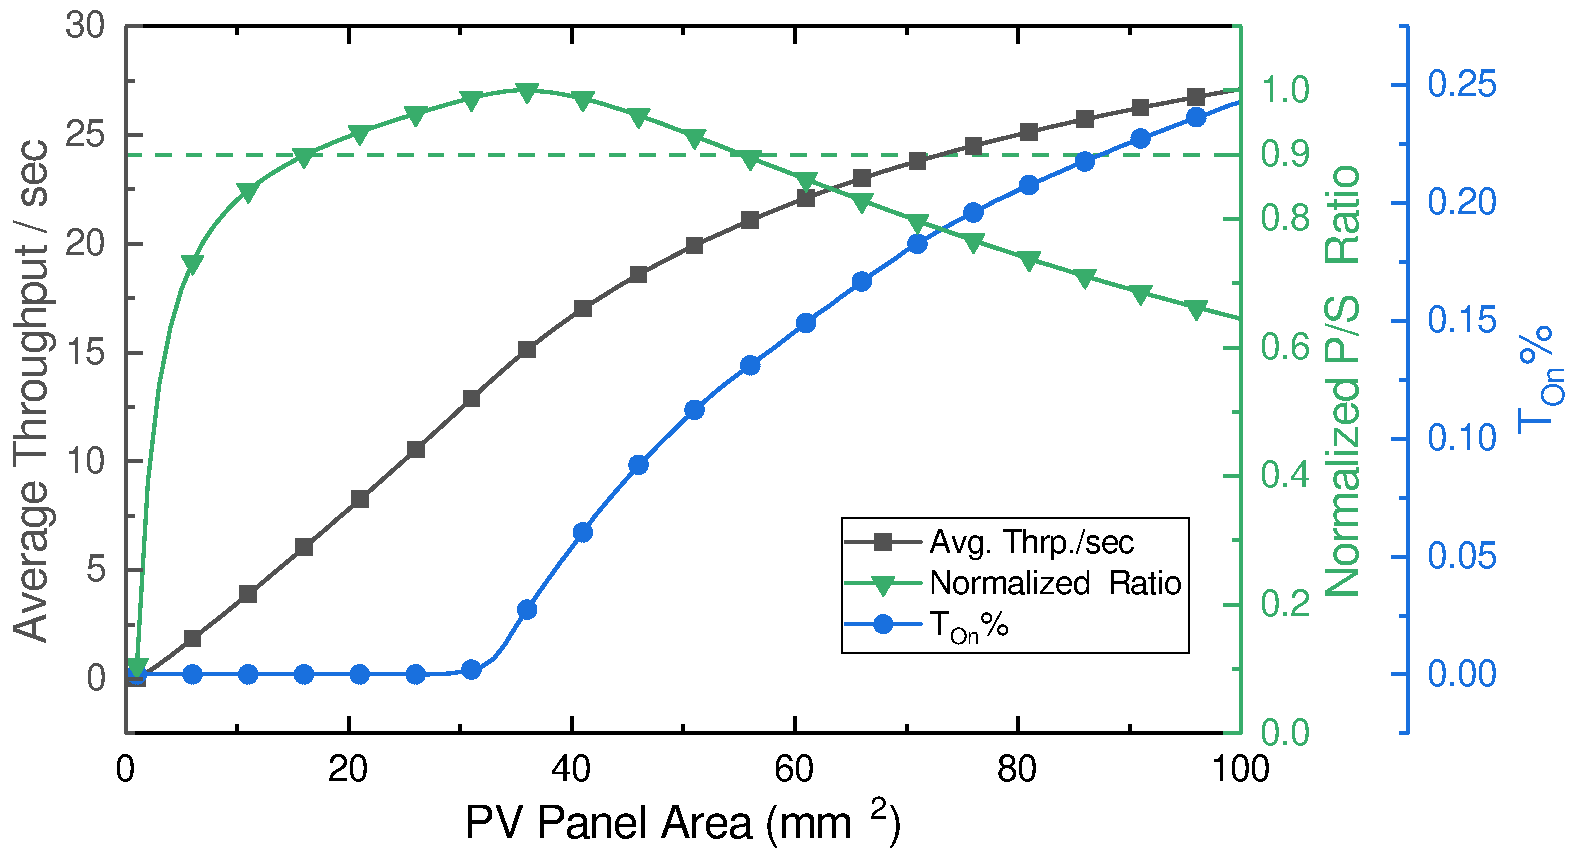
\includegraphics[width=13cm]{figure/work1/SizeHar}
    \caption{Sizing effect of energy harvester given annual outdoor solar irradiance.}
    \label{Figure:SizeHar}
\end{figure}

As shown in Figure \ref{Figure:SizeHar}, the system average performance (throughput per second) increases with the PV panel area, but the relationship is non-linear under real-world varying energy conditions. Given a small harvester (the left end of Figure \ref{Figure:SizeHar}), a large part of the harvested energy is used for compensating the system leakage, so the P/S ratio is low. Given a large harvester (the right end of Figure \ref{Figure:SizeHar}), the system spends nearly 25\% of time in the On region, which means in around half of the daytime the system could have harvested more energy; in this case, enlarging the harvester size is not "profitable". Alternative choices can be using a more powerful load if higher performance is needed or scale down the harvester size if lower performance is still beyond requirement. A harvester size that leads to nearly the maximum P/S ratio is efficient for deploying energy harvesting devices. A reference line of 90\% maximum P/S ratio is given in this figure, and designers can choose a harvester size with P/S ratio above the reference line (from 16mm$^2$ to 56mm$^2$ in this example) according to their needs for minimum performance or maximum area. Nevertheless, harvester sizes outside this range can still be chosen if needed, but that leads to an inefficient harvester deployment. 
% from 18 to 57 mm2

\subsection{Sizing storage and harvester together given real-world irradiance data} \label{Section:4.5}

After explaining the sizing effect of both energy storage and energy harvester, this section presents the combined sizing effect given real-world outdoor solar irradiance as the energy source. As shown in Figure \ref{Figure:SizeHarSto}, the performance is dominated by the energy harvester size because it largely determines how much energy can be generated. For every harvester size shown in this figure, the optimal energy storage size that delivers the best performance occurs at around 80-90\textmu F. This indicates sizing energy storage has little relationship with the energy harvester size. Within a suggested range of efficient energy harvester sizes (from 16$mm^2$ to 56$mm^2$), increasing energy storage to 80\textmu F contributes to 5.7-22.2\% execution speedup. This performance improvement by sizing storage decreases with increased harvester size, because the state management overheads account for a less percentage of the total harvested energy. 

\begin{figure}[H]
    \centering
    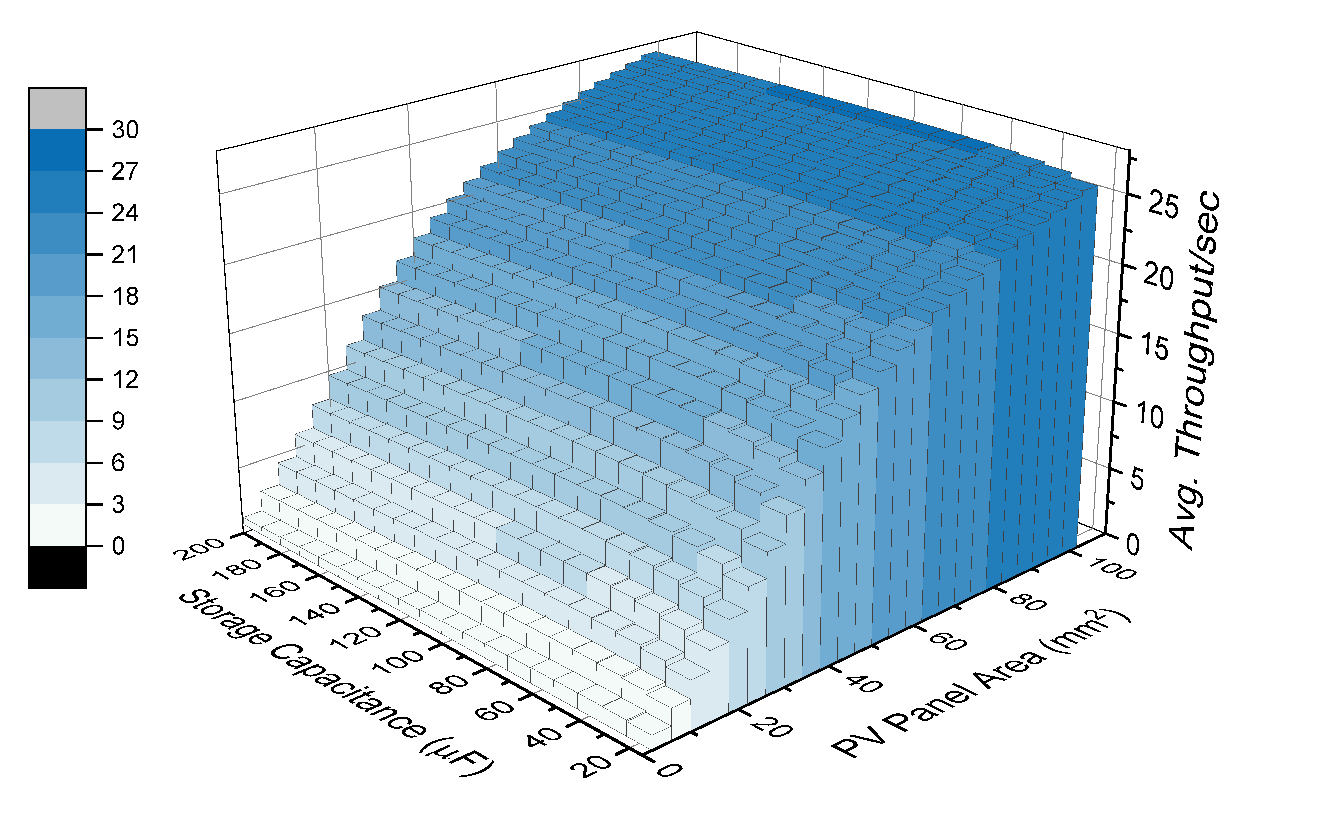
\includegraphics[width=13cm]{figure/work1/SizeHarSto}
    \caption{Effect of energy storage and energy harvester sizing on average application performance given yearly outdoor solar irradiance.}
    \label{Figure:SizeHarSto}
\end{figure} 


\section{Discussion}

Although our sizing method considers the distribution of energy conditions after deployment, the variations of energy conditions in the time domain are ignored in this sizing method. Such variations may have an impact on the short-term system behaviours. This impact may not be obvious in solar energy harvesting as the solar source is relatively stable compared to other energy sources, such as radio-frequency signals, human body movements, and acoustic energy. 

Besides the sizing concerns on performance and dimensions discussed above, published works also mention other sizing goals. Colin et al. \cite{Colin:2018:RES:3173162.3173210} propose the need to dynamically scale energy storage at run time to achieve both task atomicity (related to computing correctness in task-based intermittent computing) and execution responsiveness. Also, Jackson \cite{Jackson:2019:COC:3302506.3310400} et al. propose using novel batteries to avoid power intermittency and ensure a high completion rate for periodic workloads.


\section{Summary}

In this chapter, we presented a sizing method for energy storage and energy harvester in energy harvesting IoT deployment, with concerns on device performance and dimensions. We modelled an intermittent computing device based on outdoor solar energy harvesting, with formulations for estimating application performance from harvested power. We analysed the system behaviours of intermittent computing devices and apply our sizing method based on this model. Our sizing method gives a suggestion on energy harvester sizing that balances average performance and device dimensions. Further results show that properly sizing energy storage leads to an execution speedup by 5.7-22.2\% in the suggested range of energy harvester sizes under real-world outdoor deployment. 